\documentclass[12pt]{article}
\usepackage[margin = 1in]{geometry}
\usepackage[USenglish]{babel}
\usepackage{natbib}
\usepackage{multirow}
\usepackage{graphicx}
\usepackage{fancyhdr}
\usepackage{setspace}
\usepackage{verbatim}
\usepackage{booktabs}
\usepackage{amsmath}
\usepackage{lscape}
\usepackage{dcolumn}
\usepackage{subcaption}
\usepackage[title]{appendix}
\usepackage{xcolor}
\usepackage{todonotes}
\usepackage{titletoc}
\usepackage[colorlinks=true,citecolor=red!50!black,urlcolor=blue!50!black,linkcolor=red!50!black]{hyperref}

\author{Patrick W. Kraft\footnote{Ph.D. Student, Stony Brook University, \href{mailto:patrick.kraft@stonybrook.edu}{patrick.kraft@stonybrook.edu}.
%I thank Jennifer Jerit, Jason Barabas, Stanley Feldman, Fridolin Linder, Scott Clifford, Peter DeScioli, and participants of the Political Science Graduate Student Colloquium at Stony Brook University as well as participants at the panel of the 2015 Annual Meeting of the Midwest Political Science Association for helpful comments on earlier versions of this manuscript.
}}
\date{today}

\title{Moral Foundations of Political Reasoning\footnote{An earlier version of this paper was presented at the 73rd Annual Conference of the Midwest Political Science Association, April 16-19, 2015. The manuscript and code are available on GitHub: \url{https://github.com/pwkraft/mft}.}\\
\large{Investigating the Moral Underpinnings of Political Judgment}}
\date{\today}


\begin{document}
\maketitle
\onehalfspacing

\begin{abstract}
This paper investigates how differences in moral judgments between liberals and conservatives shape and structure political reasoning. Using open-ended survey responses in the 2012 American National Election Study, I utilize a moral dictionary proposed in the literature on Moral Foundations Theory to identify references to basic moral intuitions when individuals report their attitudes towards political parties and candidates. The results show that liberals and conservatives rely on different sets of moral foundations when evaluating political actors---even without being cued to think about morality. Furthermore, moral reasoning is shown predict important political outcomes such as attitudes towards parties and candidates, vote choice, as well as turnout, even after controlling for party identification. However, the ideological differences in moral reasoning are more context-specific than previous studies suggest.

\vspace{\baselineskip}
\noindent \textbf{Keywords:} Moral Foundations Theory, Political Reasoning, Ideology, Political Behavior, Open-ended Survey Responses
\end{abstract}
\newpage


\section{Introduction}

Moral values serve as a source of coherence in political attitudes and they shape individual belief systems. There is evidence, for example, that moral considerations predict a person's attitudes on a range of ``culture-war'' issues such as abortion and same-sex marriage above and beyond demographic characteristics and ideology (\citealt{koleva2012tracing}; also see \citealt{clifford2015concerns}). Even issues that are not considered intrinsically ``moral,'' such as those related to the economy, can be connected to underlying moral convictions \citep{ryan2014reconsidering}. Moral convictions, in turn, have been shown to reduce tolerance of divergent attitudes and lower acceptance of compromise \citep[][]{skitka2010psychology,ryan2016no}. As such, individual moral reasoning may provide important insights into the recent increase in polarization in American Politics \citep{iyengar2015fear}. According to one prominent theoretical approach, \textit{Moral Foundations Theory}, moral thinking is organized by five central ``foundations'': harm/care, fairness/reciprocity, ingroup/loyalty, authority/respect, and purity/sanctity \citep{haidt2008moral}. Liberals and conservatives differ in their relative emphasis of these foundations, with liberals prioritizing the foundations of harm/care and fairness/reciprocity, and conservatives endorsing all five foundations more or less equally \citep{graham2009liberals}. A growing body of work has documented the political relevance of moral foundations in the area of vote choice \citep{iyer2010beyond, franks2015using}, issue preferences \citep{koleva2012tracing, low2015moral, clifford2015concerns}, and candidate trait evaluations \citep{clifford2014linking}.

While we observed consistent differences between liberals and conservatives in terms of their latent emphasis on moral foundations, it is unclear whether people utilize the foundations in their day-to-day political reasoning---i.e., without being prompted by the language of a questionnaire. Previous research mostly relied on the Moral Foundations Questionnaire (MFQ) as a measure of moral reasoning, which consists of explicit judgments about the relevance of moral considerations as well as evaluations of moral judgment statements \citep[e.g.][]{graham2011mapping}. By directly asking people about the importance of considerations related to the five foundations, previous analyses presupposed an important link that requires more careful empirical investigation. This study examines whether differences in moral reasoning between liberals and conservatives manifest themselves in a more unobtrusive context (i.e., without explicitly asking people to think about morality as is done in the MFQ). Using data from the 2012 American National Election Study, I create a measure of moral reasoning based on individual responses to the open-ended likes-dislikes questions and the moral dictionary introduced by \citet{graham2009liberals}. Finding similar patterns in this context provides stronger evidence for the claim that political reasoning is influenced by basic moral intuitions. The present study therefore contributes to the literature by investigating patterns of moral reasoning among individuals where the potential connection between morality and politics is not induced or facilitated by design.

Overall, the results indicate that liberals and conservatives differ in their reliance on specific moral considerations when evaluating political parties and candidates--even without being cued to think about morality. Furthermore, moral reasoning powerfully influences political participation, candidate evaluation, and voting behavior, even after controlling for individual party identification. While the ideological differences are broadly consistent with Moral Foundations Theory, moral reasoning in the realm of politics is more context-specific than previous research suggests. From a methodological standpoint, the research presented here illustrates the advantages of open-ended survey measures for examining the antecedents of political reasoning.


%% % % % % % % % % % % % % % % % % % % % Comments Jenn
%
%To what extent are political belief systems and ideologies meaningfully structured by individual psychological characteristics and underlying motivations? This question has been of frequent scholarly interest in political science and related disciplines, yielding an array of different perspectives. Early accounts emphasized how ordinary citizens lack consistent political attitudes and knowledge necessary to form meaningful ideologies (e.g. Converse, 1964). However, with increasing levels of polarization and partisan sorting in contemporary politics (Iyengar and Westwood, 2015), there has been renewed interest in systematic psychological and attitudinal differences between liberals and conservatives (Jost, 2006). One such area of research focuses on the differing moral concerns of liberals and conservatives. According to one prominent theoretical approach, Moral Foundations Theory, moral thinking is organized by five central “foundations": harm/care, fairness/reciprocity, ingroup/loyalty, authority/respect, and purity/sanctity (Haidt and Joseph, 2008). Liberals and conservatives differ in their relative emphasis of these foundations, with liberals prioritizing the foundations of harm/care and fairness/reciprocity, and conservatives endorsing all five foundations more or less equally (Graham, Haidt, and Nosek, 2009). A growing body of work has documented the political relevance of moral foundations in the area of vote choice (Iyer et al., 2010; Franks and Scherr, 2015), issue preferences (Koleva et al., 2012; Low and Wui, 2015; Clifford, Jerit, Rainey, and Motyl, 2015), and candidate trait evaluations (Clifford, 2014).
%
%While there are consistent differences between liberals and conservatives in terms of their latent emphasis on moral foundations, it is unclear whether people utilize the foundations in their day-to-day political reasoning (i.e., without being prompted by the language of a questionnaire. Previous research has relied almost exclusively on the Moral Foundations Questionnaire (MFQ) as a measure of moral reasoning, which explicitly asks people to judge the relevance of particular moral considerations (e.g.Graham et al., 2011). But, by directly asking people about the importance of considerations related to the five foundations, previous analyses presuppose an important link that requires more careful empirical investigation. The present study addresses this gap by examining whether differences in moral reasoning between liberals and conservatives manifest themselves in a more unobtrusive context (i.e., without explicitly asking people to think about morality). Using data from the 2012 American National Election Study, I create a measure of moral reasoning based on individual responses to the open-ended likes-dislikes questions and the moral dictionary introduced by Graham, Haidt, and Nosek (2009). Finding similar patterns in this context provides stronger evidence for the claim that political reasoning is influenced by basic moral intuitions. The present study therefore contributes to the literature by investigating patterns of moral reasoning among individuals where the potential connection between morality and politics is not induced or facilitated by design.
%
%Overall, the results indicate that liberals and conservatives differ in their reliance on specific moral considerations when evaluating political parties and candidates (even without being cued to think about morality). Furthermore, moral reasoning powerfully influences political participation, candidate evaluation, and voting behavior—even after controlling for a person’s party identification. Even though the ideological differences are broadly consistent with Moral Foundations Theory, moral reasoning in the realm of politics is more context-specific than previous research suggests. [*] From a methodological standpoint, this study illustrates the value of open-ended survey measures to illuminate the antecedents of political reasoning.
%
%% % % % % % % % % % % % % % % % % % % % % % % % % % % % % % % % % % % % % % % % % % % % % % % % % % % % % % % %

\section{Theoretical Framework}

To what extent are political belief systems and ideologies meaningfully structured and constrained by individual psychological characteristics and underlying motivations? This question has been of frequent scholarly interest in political science and related disciplines, yielding an array of different perspectives. Early accounts emphasized how ordinary citizens lack consistent political attitudes and knowledge necessary to form meaningful ideologies \citep[e.g.][]{converse1964nature}. However, with increasing levels of polarization and partisan sorting in contemporary politics \citep{iyengar2015fear}, there has been renewed interest in systematic psychological and attitudinal differences between liberals and conservatives \citep{jost2006end}. One such area of research focuses on the differing moral concerns of liberals and conservatives.


\subsection{Moral Foundations Theory}

The relationship between moral values and political belief systems is a major focus of the Moral Foundations framework \citep[c.f.][]{haidt2012righteous}. Haidt and colleagues showed that liberal morals focus on ``individualizing'' foundations, which include harm/care and fairness/reciprocity. Conservatives, on the other hand, also emphasize the remaining foundations of ingroup/loyalty, authority/respect, and purity/sanctity, labeled the ``binding'' foundations \citep{haidt2007morality,graham2009liberals}.\footnote{Subsequent accounts of Moral Foundations Theory discussed the inclusion of further dimensions, such as \textit{Liberty/Oppression} \citep[c.f.][]{graham2013moral,haidt2012righteous}. However, the analyses presented here will only focus on the dimensions initially suggested in \citet{haidt2008moral}.}

Haidt and colleagues developed the Moral Foundations Questionnaire (MFQ) to measure individual differences in the emphasis of each foundation. The MFQ consists of a series of items that explicitly ask people to rate the relevance of different considerations when making decisions about right and wrong.\footnote{For example, one of the considerations is ``Whether or not some people were treated differently than others.'' High relevance of the considerations is viewed das an indicator for the fairness/reciprocity dimension (c.f. \url{http://www.moralfoundations.org/}).} The questionnaire also asks individuals to indicate their level of agreement with statements that represent the values implied by the five foundations.\footnote{For example, respondents are asked to report their agreement with the statement ``I am proud of my country’s history'' as an indicator for the ingroup/loyalty dimension.} However, \citet{graham2009liberals} did not exclusively rely on the MFQ. For example, one of their studies consisted of a quantitative analysis of sermons from liberal and conservative churches. The authors proposed a dictionary of words (and word stems) that signal references to the specific moral foundations and showed that liberal sermons were more likely to contain expressions related to harm/care and fairness/reciprocity, than conservatives \citep[see also][for multi-dimensional conceptualizations of ideology]{haidt2009above}.

Subsequent studies extended the initial findings. For example, scholars showed that moral concerns predicted attitudes towards a wide variety of divisive political issues \citep[e.g.][]{koleva2012tracing,low2015moral}. \citet{federico2013mapping} linked moral foundations to individual social dominance orientation (SDO) and right-wing authoritarianism (RWA). Further research directly investigated the relationship between moral foundations and candidate preferences \citep{iyer2010beyond} or trait inferences about candidates \citep{clifford2014linking}. Moral foundations have also been shown to predict turnout \citep{johnson2014ideology} as well as voting behavior in the 2012 US Presidential election \citep{franks2015using}.

Overall, previous research strongly supports the view that liberals and conservatives endorse different moral foundations and that these differences are related to political attitudes, evaluations, and behavior. Yet, nearly all existing work relies on the Moral Foundations Questionnaire (MFQ) as a measure of individual moral reasoning \citep[but see][]{clifford2014linking}. 


\subsection{The `Missing Link' to Political Reasoning}

Measuring moral foundations using the MFQ imposes important constraints on our theoretical conceptualization of moral reasoning and the range of hypotheses we can investigate. Most importantly, it does not allow us to directly examine the conditions under which the connection between moral values and political ideology manifests itself when citizens reason about politics and evaluate political actors. Some scholars have criticized the MFQ because it does not ask people to make moral judgments per se. Indeed, \citet[1031]{graham2009liberals} describe the reports on moral relevance as ``self-theories of moral judgment,'' rather than direct measures of judgment itself. Such abstract self-theories might, in turn, deviate from actual judgments in specific situations \citep[see][for an alternative way to measure moral judgment]{clifford2015moral}.

From a theoretical perspective, moral foundations are viewed as stable predispositions that affect attitudes and preferences regardless of potential individual differences and contextual effects. However, the incorporation of moral considerations in a specific political context could be much more variable. Previous research suggests that campaigns and elite communication can have important influences on individual moral reasoning. For example, \citet{clifford2013words} found that at the elite level, proponents and opponents of stem cell research place distinctive weights on moral foundations which in turn affected the public attitudes and the underlying considerations related to the issue. A subsequent study showed that elite rhetoric plays an important role in linking individual moral foundations with political attitudes, but only for those individuals who were most likely be exposed to it (\citealt{clifford2015concerns}; also see \citealt{day2014shifting}). While these studies do not contradict Moral Foundations theory, they cast some doubt on the notion that moral reasoning in politics is as a direct reflection of stable moral intuitions. 

The literature on \textit{moral convictions} further suggests that moral reasoning in the realm of politics can be more variable than proposed by MFT. Skitka and colleagues argue that individuals hold moralized attitudes if they have a universal perception of ``right and wrong'' connected to the issue at hand \citep{skitka2005moral,mullen2006exploring,skitka2010psychology}. This view implies that there can be considerable variance in the degree to which moral considerations are raised between individuals and across issues.

Research on moral conviction and moral foundations developed largely independent of each other, which can be partly explained by the fact that the measurement approaches in both fields are not directly compatible. Moral foundations are measured as general predispositions that are implicitly assumed to apply in any context, whereas convictions are intrinsically linked to individual attitudes about specific issues. Moving beyond the MFQ and measuring moral reasoning as the explicit expression of foundations can help us to bridge the gap between both literatures. If we assume that moral convictions can be expressed as moral considerations that overlap with the moral taxonomy developed in the Moral Foundations literature, then the variability in moral reasoning measured through open-ended responses can be informative for the degree to which political attitudes are infused by moral convictions.

Overall, individuals who are exposed to the political process and resulting elite communications are expected to be more likely to incorporate moral considerations in their political reasoning. Individuals who are not engaged in politics, on the other hand, might focus on other considerations when thinking about and forming their political preferences. The extent to which individuals rely on moral considerations when evaluating political actors is therefore not necessarily stable among individuals and across contexts. Rather, the tendency to emphasize moral foundations may be contingent upon individual levels of political sophistication, media exposure, and political discussions.\footnote{However, some studies indicate that individuals make frequent references to values when discussing their policy preferences \citep{feldman1992political} and that the reliance on basic values is not contingent on individual characteristics such as political sophistication \citep[e.g.][]{goren2001core,goren2004political,marietta2007values}.} The degree to which political attitudes are moralized as well as the ideological differences in moral reasoning could not be investigated by relying solely on MFQ and related measures. Instead, it is necessary to differentiate between moral \textit{foundations} as stable predispositions, and moral \textit{reasoning} as the actual reliance on specific moral considerations and arguments, both from a theoretical as well as a measurement perspective. Previous research in moral foundations theory largely neglected this difference.



\section{Empirical Analyses}

\subsection{Overview and Hypotheses}

Insofar as moral intuitions play a role in political reasoning, citizens should rely on the moral foundations when reporting their attitudes towards political actors, even if they are not explicitly asked to do so. Thus, the first step of the analyses will be to replicate the findings connected to moral foundations and ideology using open-ended survey responses:

\vspace{0.3cm}
\begin{tabular}{lp{12cm}}
\textsl{Hypothesis 1:} & Liberals will be more likely to spontaneously mention the moral foundations of harm/care and fairness/reciprocity  than conservatives when evaluating political parties and candidates. Conversely, conservatives will be more likely to emphasize moral foundations of ingroup/loyalty, authority/respect, and purity/sanctity than liberals.
\end{tabular}
\vspace{0.5cm}

The present study contributes to the literature by clarifying the role of the foundations in day-to-day reasoning. Rather than being viewed as stable predispositions, individuals are expected to differ in the degree to rely on moral considerations in the realm of politics depending on their exposure to political discourse. I therefore argue that the use of the moral foundations is more variable and context specific than previous research on Moral Foundations theory suggests; more specifically:

\vspace{0.3cm}
\begin{tabular}{lp{12cm}}
\textsl{Hypothesis 2a:} & Individuals who are more exposed to political discourse will be more likely to emphasize moral foundations when evaluating political parties and candidates than those who have less experience and are less politically engaged. \\
\textsl{Hypothesis 2b:} & Ideological differences in the emphasis on moral foundations will be more pronounced for individuals who are more engaged in the political system than those who have less experience and are less politically engaged.
\end{tabular}
\vspace{0.5cm}

This hypothesized variability in moral reasoning, measured through open-ended responses, is expected to be politically consequential. First of all, the differences in the degree to which each foundation is emphasized should directly affect political preferences and vote choice. Furthermore, previous work on moral conviction suggests that individuals who hold moralized attitudes are more likely to engage in politics, are less accepting of divergent positions and compromise, and show stronger emotional and affective responses related to the respective issues. If individuals express their moral convictions by referencing considerations related to the foundations identified by Haidt and colleagues, we would expect that general moral reasoning affects political participation and related measures of interest. As such, variance in moral reasoning, which cannot be captured by relying solely on measures like the MFQ, is politically relevant and is expected to have a measurable impact on a variety of political outcomes:

\vspace{0.3cm}
\begin{tabular}{lp{12cm}}
\textsl{Hypothesis 3a:} & References to individual moral foundations predict candidate and party preferences, as well as vote choice, even after controlling for (strength of) party identification. \\
\textsl{Hypothesis 3b:} & The degree to which individuals rely on general moral reasoning predicts turnout and other forms of political participation, even after controlling for (strength of) party identification.
\end{tabular}
\vspace{0.5cm}


\subsection{Data, Variables, and Model Specification}

The analyses presented here are based on the 2012 American National Election Study, which contains two representative cross-sectional samples. One sample was conducted by computer assisted face-to-face interviews while the other sample is based on an internet panel group. Both samples are pooled in the analyses. While each consisted of a pre-election and a post-election wave, most items described below are drawn from the pre-election wave.\footnote{The open-ended items were included only in the pre-election wave. Accordingly, wherever possible, the set of explanatory variables was limited to the pre-election wave.}

The major dependent variables are based on open-ended questions in which respondents were asked to report what they \textit{liked} and \textit{disliked} about either presidential candidate as well as the Republican and Democratic parties. More specifically, respondents were asked to list anything in particular that they like/dislike about the Democratic/Republican party as well as anything that might make them vote/not vote for either of the Presidential candidates and were probed by the interviewer asking ``anything else?'' until the respondent answered no. All open-ended responses were pre-processed by correcting spelling errors using an implementation of the Aspell spell checking algorithm in \texttt{R} (\url{www.aspell.net}), and deleting individuals who responded in Spanish. 

Our goal is to use the open-ended responses to identify the extent to which respondents relied on specific moral foundations when talking about their political attitudes and preferences. Previous studies in the domain of Moral Foundations Theory relied on the dictionary proposed by \citet{graham2009liberals} to identify such references to moral dimensions \citep[e.g.][]{clifford2013words}.\footnote{The dictionary provided by \citet{graham2009liberals} is also presented in Appendix~\ref{app:oview}.} For example, words like ``protect'' and ``suffer'' indicate references to the harm/care foundation, ``equality'' and ``tolerant'' signal reasoning based on the fairness/reciprocity foundation, ``patriot'' and ``betrayal'' indicate reference to the ingroup/loyalty foundation, ``honor'' and ``respect'' signal considerations related to authority/respect, whereas ``integrity'' and ``duty'' indicate reference to the purity/sanctity foundation. Conventional dictionary-based methods consist of dichotomous indicators, simple counts, or proportions of signal word occurrences for each dictionary category in each text or response.

But what if the content of the dictionary itself is not perfectly suited for our purposes? While \citet{graham2009liberals} developed the word lists as a collection of general associations related to the base foundations that could be applied in any context, some words included in the lists might be problematic when applied to the open-ended responses considered here. More specifically, individual words appear to be too ubiquitous in the realm of politics and candidate evaluations to be regarded as an unambiguous indicator for specific moral considerations. For example, the moral foundations dictionary includes ``leader'', ``respect'', ``law'', and ``illegal'' as a signal words for the authority/respect dimension. If respondents are asked about their attitudes towards both presidential candidates, they might be inclined to describe them as good or bad \textit{leaders} irrespective of factual moral considerations.

One way to address this problem would be to revise the dictionary. However, this leaves a lot of discretion to the researcher and creates the potential issue that signal words are chosen based on ex-post reasoning about individual response behavior in the given context. Instead, I rely on techniques developed in the fields of information retrieval to match search queries to relevant text documents \citep[see][for an introduction]{manning2008introduction}. Consider the example of a political scientist who searches for articles containing the keywords ``morality'' and ``politics'' on Google Scholar. Should the search engine consider both terms as equally important when searching for matches in the text documents? Arguably, there are many more instances of ``politics'' than of ``morality'' in academic articles on Google Scholar. If we were to simply sum up the number of matches for each document, we would end up identifying a lot of documents that are, in fact, too general (i.e. that only discuss ``politics''). In order to identify the set of most relevant documents, it makes sense to increase the importance of keywords that appear in fewer documents (i.e. ``morality''), since they carry more discriminative information.

I rely on the same logic to create a measure that represents the degree to which a person's open-ended response resembles Graham et al.'s \citeyearpar{graham2009liberals} dictionaries for each moral dimension (referred to below as ``similarity score''). Formally, similarity is the tf-idf cosine score\footnote{The acronym tf-idf stands for ``term frequency - inverse document frequency''. It refers to the rationale that the frequency of specific terms are weighted by the inverse of the frequency of occurrence across documents.} between the dictionaries and a person's response to the open-ended items on the ANES. A technical discussion appears in Appendix~\ref{app:measure}, but the measure has several useful properties that I note here. Most importantly, words that appear in nearly all open-ended remarks affect similarity less than the words that are mentioned only by few respondents (because ubiquitous words convey less information about differences across individuals). A related property of the measure is that words that are mentioned multiple times in a response are weighted more than words that only appear once. Similarity is a continuous measure that ranges between 0 (no overlap between dictionary and response) and 1 (response is identical to dictionary), and is independent of response length.

Overall, the similarity score provides a correction for potential distortions due to suboptimal terms in the dictionary while leaving its exact content outside of the researcher's discretion. While the resulting measure theoretically ranges from 0 to 1, we only observe very low values since open-ended responses are quite distinct from the dictionaries. Since the exact values do not have a straightforward interpretation\footnote{Technically, values on this variable describe the cosine of the angle between the tf-idf vector space representation of the dictionary and each open-ended response. Please refer to the Appendix~\ref{app:measure} for a more detailed discussion.}, the measure for each moral dimension is mean-centered and rescaled to unit variance.

Respondents were not included in the analysis if they failed to provide an answer in all open-ended items, or if the interview language was Spanish. Table~\ref{tab:appB1mis} in the appendix provides an overview over the number of omitted cases. About 4\% of the interviews were held in Spanish and about 7\% of the respondents did not provide any open-ended response. Furthermore, Figure~\ref{fig:appB2num} in the appendix displays histograms of the length of the respondents' answers to all open-ended items. On average, the collection of all open-ended responses consists of about 75 words for each individual.

Individual response patterns are modeled via seemingly unrelated regression (SUR) of the rescaled tf-idf cosine scores for each of the moral foundations under consideration. The SUR framework allows us to account for the fact that error terms between different moral dimensions might be correlated. The key independent variable used to predict the emphasis on each of the moral foundations, is \textit{political ideology}. Respondents were asked to place themselves on a seven-point scale ranging from extremely liberal to extremely conservative. Since there is no reason to suggest that moderates should fall in between liberals and conservatives in terms of their moral foundations (i.e. that the relationship between `continuous' ideological self-placement and the likelihood to mention specific moral foundations is inherently linear), I constructed dichotomous variables indicating whether respondent identified as liberals, conservatives, or moderates.

Additional control variables included in the analyses are \textit{church attendance}, \textit{education} (college degree), \textit{age}, \textit{sex}, \textit{race} (African American), as well as the overall length of the individual responses in the open-ended questions (\textit{number of words}). The inclusion of the length of individual responses as control variables should account for potential confounding factors such as general effects of increased political literacy on the complexity of open-ended responses.

Other factors that are expected to be related to references to moral foundations include \textit{political sophistication}, which was measured as the sum of correct answers to objective knowledge questions. The analysis also investigates the effect of \textit{political media exposure} as well as the frequency of \textit{political discussions} with friends and family members. Here, we not only look at the influence on individual foundations, but also examine whether these factors influence \textit{general} moral reasoning. This variable is measured as the sum of individual similarity scores (again, values are mean centered and standardized to make them directly interpretable). It can be interpreted as a aggregate measure of how much respondents emphasize any moral consideration in their responses.

In order to examine the relevance and consequences of moral reasoning, the similarity scores for each of the moral foundations are used as independent variables to predict political outcomes. The dependent variables considered here are \textit{candidate} and \textit{party evaluations} (measured as the respective feeling thermometer differentials), as well as \textit{voting behavior} (measured as a dichotomous indicator of vote choice for the Democratic rather than the Republican Presidential candidate). Furthermore, we investigate whether general moral reasoning (measured as the sum of similarity scores) affects retrospective \textit{turnout}, as well as dichotomous indicators for participation in demonstrations, wearing campaign buttons, and signing petitions. Finally, in addition to the controls discussed previously, the analyses include measures of \textit{party identification} (or the strength of party identification when appropriate).



\subsection{Results}

\subsubsection{Ideological Differences in Moral Reasoning}

Figure~\ref{fig:1prop} provides an overview over the response patterns for individuals who identified as liberals, conservatives, or moderates. For each group, the figure displays the (weighted) proportion of respondents who mentioned words that were included in the five different moral foundations dictionaries as well as their 95\% confidence intervals. In order to calculate these proportions, all responses to the eight open-ended like/dislike questions (evaluating both parties and both candidates) were aggregated for each individual. Therefore, each proportion indicates the percentage of individuals who mentioned a signal word belonging to the respective moral foundation in any of his or her open-ended responses evaluating the parties or candidates.

\begin{figure}[h]\centering
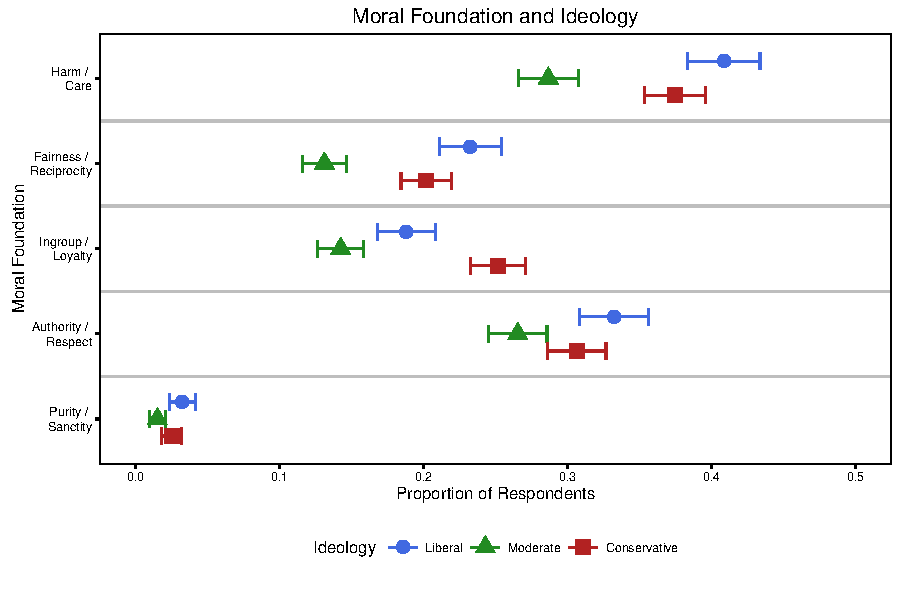
\includegraphics[scale=.9]{../calc/fig/fig1prop.pdf}
\caption{Weighted proportion of Respondents mentioning each of the moral foundations in any of their open-ended responses, along with 95\% confidence intervals. Additional plot including 2008 data is shown in the appendix, Figure~\ref{fig:appC1prop}}\label{fig:1prop}
\end{figure}

The patterns are largely consistent with theoretical expectations. Liberals were more likely than conservatives or moderates to mention the harm/care foundation. Almost half of the respondents identifying as liberals mentioned words belonging to the harm/care category in their responses. Furthermore, they were more likely than conservatives to mention the fairness/reciprocity foundation. This pattern is consistent with Moral Foundations Theory, as is the tendency for a greater proportion of conservatives to reference the ingroup/loyalty foundation than liberals or moderates. There were some notable contradictions, however. Fewer liberals used fairness/reciprocity words than authority/respect words. Indeed, the proportion of liberal respondents referencing authority/respect is almost identical to the proportion of conservatives mentioning authority/respect.

The fact that the purity/sanctity foundation was almost never mentioned by any of the respondents is surprising, since other studies found that the purity/sanctity foundation plays a very important role when looking at ideological differences \citep{koleva2012tracing}. This result suggests that subsequent analyses of survey responses might necessitate a revision of the moral foundation dictionary, since the terms contained in the dictionary might not be relevant for political evaluations. Accordingly, some of the words (e.g. in the case of purity/sanctity) are too uncommon in the political context. Due to the very rare mentioning of the purity/sanctity dimension, the subsequent analyses will concentrate on the remaining four moral foundations.\footnote{Unfortunately, this issue cannot not be properly addressed by relying on tf-idf cosine scores. The weighting can correct for some distortions due to individual ubiquitous terms in the dictionaries, but it cannot compensate for the fact that the purity dictionary as a whole only contains words that are almost never mentioned by respondents.}

Overall, these results provide an inconclusive picture on the moral foundations of political reasoning. While most patterns are consistent with our theoretical expectations, the findings for the authority/respect dimension contradict Moral Foundations Theory.\footnote{Instead of looking at the aggregation of all survey items, we can also investigate the patterns in smaller subsets of responses (see Appendix~\ref{app:desc}). For example, taking into account only open-ended responses related to the evaluations of parties \textit{or} candidates shows the same basic patterns as in the pooled analysis. The appendix additionally presents the same results based on the 2008 ANES.} However, part of the inconsistencies might be attributed to the issues with the dictionaries discussed above (i.e. ubiquitous words and differences in individual response length). In order to alleviate this concern, we now turn to the analyses of the similarity scores as measures of moral reasoning.

I estimated a set of seemingly unrelated regression (SUR) models using ideology (and the control variables discussed above) to predict the individual similarity score for each of the moral foundations (excluding purity/sanctity).\footnote{The full regression results for this and all subsequent models discussed the remainder of the paper are presented in Appendix~\ref{app:tables}.} Figure~\ref{fig:2ideol} displays the expected change in similarity with each moral foundation for liberals and conservatives holding all other variables constant at their respective means. Like the analyses in Figure~\ref{fig:2ideol}, the responses for each individual were collapsed such that the dependent variables indicate similarity with moral foundations in the collection of all open-ended likes and dislikes.

\begin{figure}[h]\centering
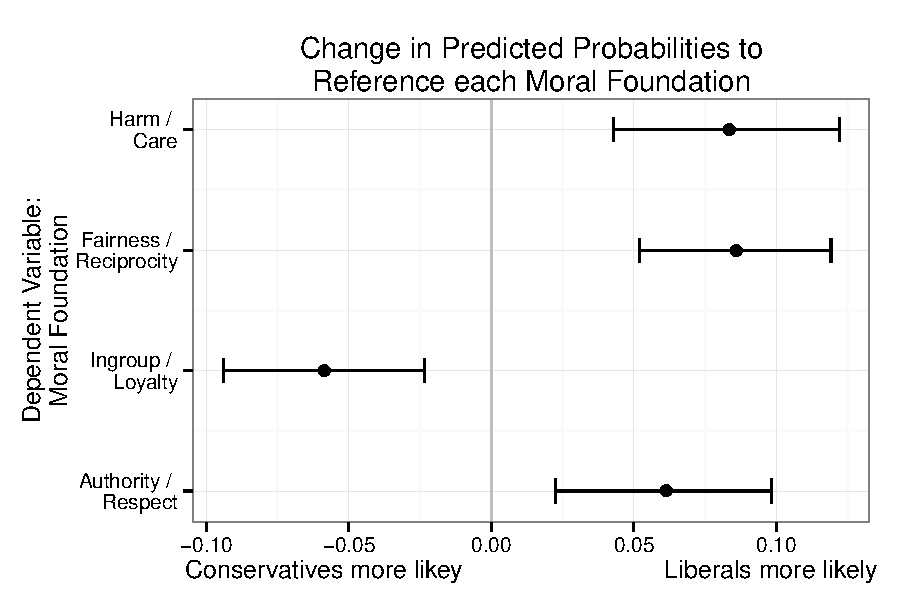
\includegraphics[scale=.9]{../calc/fig/fig2ideol.pdf}
\caption{Difference in similarity score for each moral foundation between liberals and conservatives, holding all other control variables at their respective means (along with 95\% confidence intervals). Positive values indicate that liberals emphasize the respective moral foundations more than conservatives, and vice versa. Estimates are based on seemingly unrelated regressions for each foundation's similarity score1. Additional plot including 2008 data is shown in the appendix, Figure~\ref{fig:appD1ideol}, and full model results are displayed in Table~\ref{tab:m2ideol}.}\label{fig:2ideol}
\end{figure}

Positive values denote a higher similarity score for the respective moral foundation of a response among respondents who identified as liberals, while negative values indicate a higher score among conservatives. The effects are consistent with the first hypothesis for three out of four moral foundations. Liberals emphasize the foundations of harm/care and fairness/reciprocity significantly more when evaluating political parties and candidates than conservatives. The similarity score for the harm/care foundation is about 0.15 standard deviations higher among liberals than conservatives. The effect is slightly larger for the fairness/reciprocity dimension. Conversely, being conservative increases the similarity score for the foundation of ingroup/loyalty by about 0.1 standard deviations. For the authority/respect dimension, we now see an effect in the expected direction (i.e. conservatives have higher similarity scores). However, the estimated difference between liberals and conservatives on this dimension is only small and does not reach conventional levels of significance.

I conducted auxiliary analyses to probe the robustness of the patterns in Figure~\ref{fig:1prop} and \ref{fig:2ideol} (detailed results are included in Appendix~\ref{app:robust}). As a first step, I replicated the analyses using the 2008 ANES (see Figure~\ref{fig:appD1ideol}). Overall, there are fewer patterns that are consistent with Moral Foundations Theory in 2008 than in 2012. Indeed, the only difference between liberals and conservatives that is significant is the similarity score for the ingroup/loyalty foundation. One explanation for the inconsistency across years is the fact that the open-ended responses were recorded in a more indirect manner in 2008. Many responses in 2008 consist of the interviewer's summaries of the responses in verbatim.\footnote{For example, a response in the 2008 ANES describing what the respondent likes about the Republican candidate is recorded as follows: ``his views more or less on politics, R feels he knows alot about the issues in politics
[sic]''. On the other hand, a response for the same question in the 2012 ANES was recorded as: ``I think he is honest; he couldn't do a worse job; he understands business; he understands the American people and he understands our foreign relations with Israel//He understands how much we need our military; not for war but for peace. You need to be strong to have peace//He believes in God, very important. He believes in family. He believes in dignity. the human spirit// [sic]''. While some responses in 2008 were of better quality than the example presented here, the overall proportion of summarized responses is higher than in the 2012 data. As such, the average response length is shorter in 2008 than in 2012 (c.f. Figure~\ref{fig:appB2num} in the appendix).} The sample size in 2008 also is much smaller, which explains the higher uncertainties around the estimated proportions.

One might be concerned about the decision to model the response patterns via SUR since the similarity scores are censored at zero for respondents whose response does not overlap with a dictionary. Several alternative model specifications were tested to examine whether censoring affects the results discussed thus far. First, I estimated separate Tobit models for each moral dimension. While Tobit regression accounts for the censoring in the dependent variable, it invokes the implicit assumption that error terms between equations are uncorrelated. Alternatively, responses for each individual dimension could be modeled as following a Beta distribution (which ranges from 0 to 1). However, this model again assumes independence between response patterns for each of the moral foundations. As such, it is preferable, to model the overall response pattern (i.e. for all foundations combined, including residual category) as following a Dirichlet distribution (which is, in fact, the multivariate generalization of the Beta distribution). Estimates for the robustness checks are included in the Appendix~\ref{app:robust}. The substantive results remain unchanged.

Taken together, the results indicate that there are important differences between liberals and conservatives in their reliance on different moral considerations when evaluating political parties and candidates. However, the patterns are not unequivocally consistent with the predictions of Moral Foundations Theory. The fact that some foundations showed insignificant patterns, as well as the failure to replicate the findings across years suggests that the reliance on moral foundations might be more context-specific than previously theorized.


\subsubsection{Determinants of Moral Reasoning}

Having shown that liberals and conservatives differ with regard to the moral foundations they emphasize when evaluating political actors, I next investigate whether the overall reliance on moral considerations is a product of exposure to political discourse. Therefore, I regress the sum of similarity scores for each individual on political sophistication, political media exposure, and frequency of political discussions. Figure~\ref{fig:3learn} depicts the respective effects when each independent variable (knowledge, media exposure, discussion) is increased from its empirical minimum value to its empirical maximum value, holding all other variables (including the number of words in each individual response) constant at their means.\footnote{Results for the 2008 replication of this as well as all subsequent analyses discussed in the remainder of paper are displayed in Appendix~\ref{app:robust}.}

\begin{figure}[h]\centering
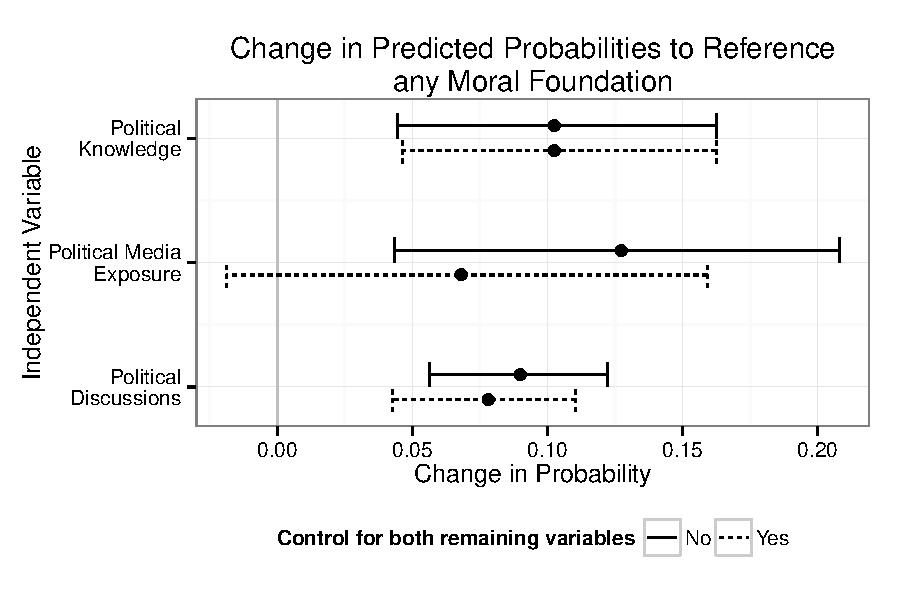
\includegraphics[scale=.9]{../calc/fig/fig3learn.pdf}
\caption{Change in predicted overall reliance on moral foundations depending on political knowledge, media exposure, and frequency of political discussions. The plot shows the predicted difference in the summed similarity scores if each of the independent variables is increased from its minimum to its maximum value holding all other variables constant at their respective means (along with 95\% confidence intervals, based on robust standard errors). Positive values indicate higher emphasis of any moral foundation. Estimates are based on OLS and dotted lines indicate estimates while controlling for both remaining variables. Additional plot including 2008 data is shown in the appendix, Figure~\ref{fig:appD7learn}, and full model results are displayed in Table~\ref{tab:m3learn}.}\label{fig:3learn}
\end{figure}

The results show that all three variables have a positive effect on the individual emphasis on moral foundations when evaluating political parties and candidates. Higher political sophistication, higher exposure to political media and news, as well as more frequent political discussions increase the degree to which individuals rely on moral considerations. Thus, citizens \textit{learn} to embed moral reasoning in their political evaluations. While moral intuitions themselves might well be innate, the extent to which individuals make use of these intuitions when thinking about politics and evaluating political actors may be more context-dependent and subject to individual heterogeneity.

The significant positive effect of frequent political discussions (even after controlling for the two remaining variables, political knowledge and media exposure), is especially interesting in this context. Citizens, who engage in frequent political arguments are more likely to use moral considerations when evaluating candidates and parties. This result suggests that morality serves as a rhetorical tool utilized to convince others of certain political views.

In addition to examining the reference to moral foundations \textit{in general}, we can also consider whether the effects of political discourse increase the differences in the emphasis on specific dimensions between liberals and conservatives. Figure~\ref{fig:4ideolearn} presents the change in the effect of ideology on the individual similarity scores moderated by political knowledge, media exposure, and frequency of political discussions. Thus, each point in the figure displays the interaction effect between knowledge (or media exposure, or discussion) and ideology as a difference-in-difference in predicted similarity holding all other variables constant at their respective means. For example, the positive effect for political knowledge on the similarity score for harm/care (top left part in the figure) indicates, that when political knowledge is increased from its empirical minimum to its maximum, the difference between liberals and conservatives is increased such that the average similarity with the harm/care foundation is about 0.5 standard deviations higher for liberals than for conservatives. In other words, positive effects imply that the gap between liberals and conservatives on the respective dimension is increased in favor of liberal respondents. Negative effects, on the other hand, indicate that the gap between liberals and conservatives is increased with conservatives showing stronger emphasis of the respective moral dimension.

\begin{figure}[h]\centering
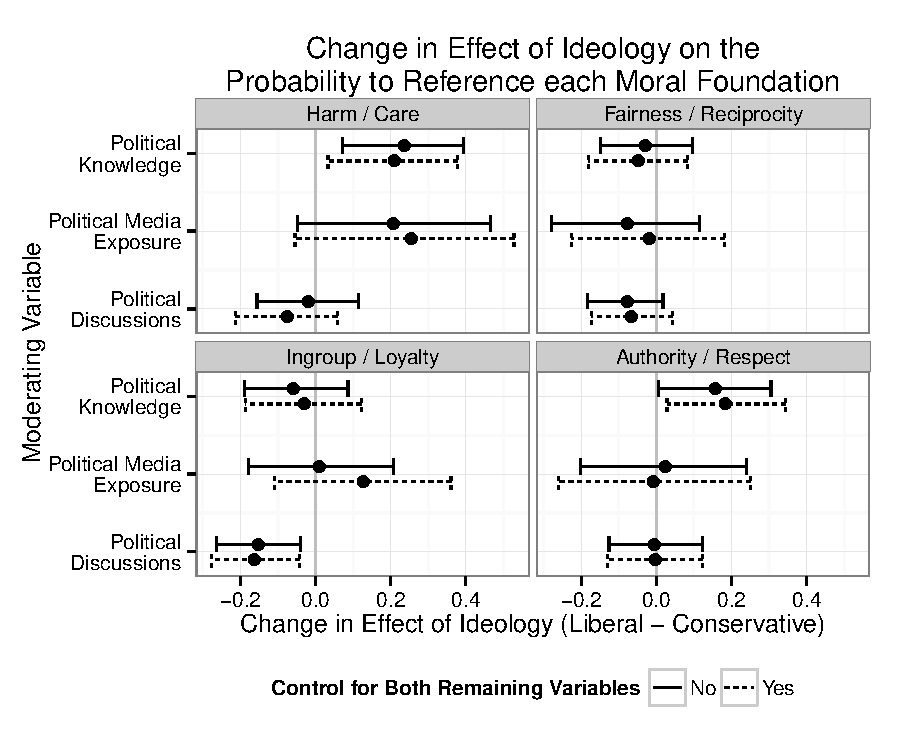
\includegraphics[scale=.9]{../calc/fig/fig4ideolearn.pdf}
\caption{Change in effect of ideology on emphasis of each moral foundation moderated by political knowledge, media exposure, and frequency of political discussions (difference-in-difference). The plot shows how the difference in predicted similarity scores for each moral foundation between liberals and conservatives changes if each of the independent variables is increased from its minimum to its maximum value holding all other variables constant at their respective means (along with 95\% confidence intervals). Positive values indicate that liberals are more likely to mention a specific moral foundation if they score high on the moderating variable (knowledge, exposure, or discussions), and vice versa. Estimates are based on individual OLS models for each foundation and dotted lines indicate estimates while controlling for both remaining variables. Additional plot including 2008 data is shown in the appendix, Figure~\ref{fig:appD8ideolearn}, and full model results are displayed in Tables~\ref{tab:m4ideolearn2012a} to \ref{tab:m4ideolearn2008b}.}\label{fig:4ideolearn}
\end{figure}

In order to interpret these difference-in-difference effects, consider again the basic findings reported in Figure~\ref{fig:2ideol}. The estimates showed that on average, liberal responses were more similar to the foundations of harm/care and fairness/reciprocity, whereas conservative responses were more similar to the ingroup/loyalty dimension. Turning to Figure~\ref{fig:4ideolearn}, we see that for individuals with high political knowledge and media exposure, the difference between liberals and conservatives in terms of the harm/care foundation was more pronounced: the difference between liberals and conservatives is increased such that liberals are even more likely to reference this dimension compared to conservatives. While we do not observe any meaningful moderation effects for the fairness/reciprocity dimension, there is some evidence that the ideological gap in the ingroup/loyalty dimension is higher for respondents who discuss politics more frequently.

Overall, political knowledge, media exposure, and political discussions do not only affect general levels of moral reasoning but also moderate the ideological gap between liberals and conservatives. This finding indicates that the effects of political discourse cannot be reduced to an artefact of differences in political literacy and more elaborate argumentation. Some portion of the ideological differences in emphasis on moral foundations can therefore be described as a product of learning in the political environment.
\clearpage


\subsubsection{Consequences and Political Relevance of Moral Reasoning}

Previous research relying on the MFQ has linked moral foundations to an array of political outcomes, such as turnout \citep{johnson2014ideology}, candidate preferences \citep{iyer2010beyond}, and voting behavior \citep{franks2015using}. But do we see the same patterns for explicit moral reasoning as compared to latent moral foundations? As a first step, we will examine whether references to moral foundations affect political participation.

\begin{figure}[h]\centering
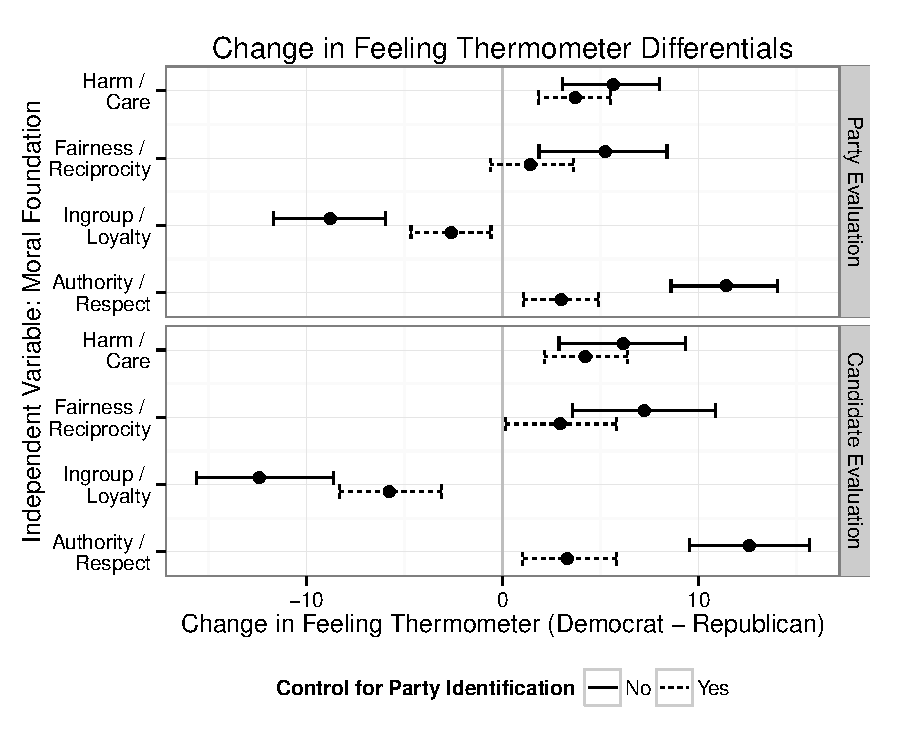
\includegraphics[scale=.9]{../calc/fig/fig7feel.pdf}
\caption{Change in predicted feeling thermometer differential when similarity score is increased from its minimum (no overlap between dictionary and response) by one standard deviation, holding all other control variables constant at their respective means (along with 95\% confidence intervals). Positive values indicate that respondents who emphasized the respective foundation evaluated the Democratic candidate/party more favorably than the Republican candidate/party, and vice versa. Estimates are based on a single OLS model (using robust standard errors) including similarity scores for each foundation and dotted lines indicate estimates while additionally controlling for party identification. Additional plot including 2008 data is shown in the appendix, Figure~\ref{fig:appD11feel}, and full model results are displayed in Table~\ref{tab:m7feel}.}\label{fig:7feel}
\end{figure}

In the next step, we turn to the relationship of moral reasoning and political preferences themselves. Figure~\ref{fig:7feel} presents the results of linear regressions of similarity scores for moral foundations predicting the change in the feeling thermometer differential between the Republican and the Democratic Presidential candidate (top part of the figure) and the change in the feeling thermometer differential between the Republican and Democratic party. Positive values indicate more favorable evaluations for the Democratic candidate or party and negative values indicate more favorable evaluations of the Republican candidate or party. The patterns are largely consistent with the previous results on ideological differences. Individuals who emphasize considerations related to harm/care, and fairness/reciprocity evaluate the Democratic candidates on average between 1 and 4 points higher than the Republican candidates (on a 100 point scale). On the other hand, if individuals emphasized the ingroup/loyalty dimension, they reported stronger preferences for the Republican candidates. These effects are robust after controlling for individual party identification. Thus, in both analyses in Figure~\ref{fig:7feel}, we observed sizable and significant effects for the influence of moral reasoning.

This result is noteworthy given that respondents were not explicitly asked about morality. Furthermore, it is not necessary to distinguish between responses for either party or between positive and negative statements in order to recover meaningful patterns. Even though we are simply looking at moral reasoning in the collection of all positive and negative statements about both candidates and parties, we observe consistent and substantial effects on subsequent evaluations. The moral considerations evoked by respondents allow us to make inferences about their political attitudes and behavior irrespective of the specific party or candidate they are evaluating.

Figure~\ref{fig:8vote} presents the changes in expected probabilities of voting for the Democratic (vs. the Republican) presidential candidate in the 2012 election for individuals emphasizing the moral foundations in their open-ended responses. The estimated probabilities are based on logit models including similarity scores for each moral foundation as independent variables as well as several sociodemographic control variables, which were held constant at their mean values when calculating expected values.

\begin{figure}[h]\centering
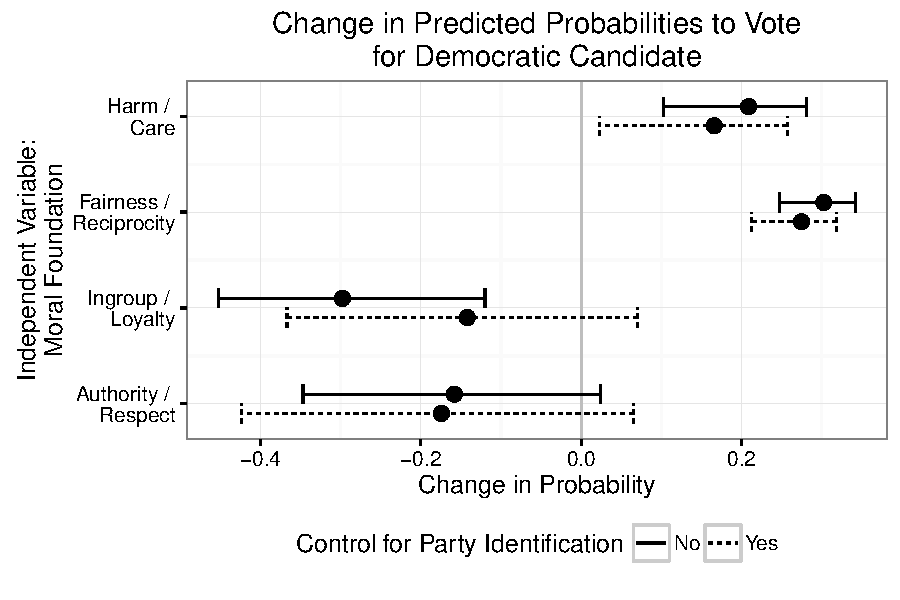
\includegraphics[scale=.9]{../calc/fig/fig8vote.pdf}
\caption{Difference in predicted probabilities to vote for Democratic candidate when similarity score is increased from its minimum (no overlap between dictionary and response) by one standard deviation, holding all other control variables constant at their respective means (along with 95\% confidence intervals). Positive values indicate that respondents who emphasize the respective foundation are more likely to vote for the Democratic candidate, and vice versa. Estimates are based on a single logit model including similarity scores or each foundation and dotted lines indicate estimates while additionally controlling for party identification. Additional plot including 2008 data is shown in the appendix, Figure~\ref{fig:appD12vote}, and full model results are displayed in Table~\ref{tab:m8vote}.}\label{fig:8vote}
\end{figure}

Again, the patterns are strikingly similar to the results presented thus far. Individuals who emphasized moral considerations related to the harm/care and fairness/reciprocity foundations are more likely to vote for Barack Obama than for Mitt Romney. Respondents who emphasized the ingroup/loyalty foundation, on the other hand, were less likely to vote for Obama. Again, these results are largely consistent with Moral Foundations Theory, although not all effects are statistically significant (especially regarding the authority/respect dimension). Overall, Figure~\ref{fig:8vote} shows that it is possible to predict voting behavior simply by observing the moral dimensions of the respondents' political reasoning, without taking into account which candidate they described, and whether the description is framed positively or negatively. Moreover, these effects largely persist after controlling for individual party identification.

So far, the results are broadly consistent with Moral Foundations theory. However, they also suggest that there is more variability in the degree to which individuals engage in moral reasoning when thinking about politics. One potential theoretical explanation for this variability could be the fact that individuals differ in the degree to which they moralized their political attitudes, which itself could be a product of exposure to political discourse. Previous research in moral convictions connected moralized attitudes to higher degrees of engagement and participation \citep{skitka2010psychology}. As such, if we assume that the expression of moral foundations in open-ended responses signals moralization and moral mandates about politics, we could expect that the overall tendency to engage in moral reasoning is related to political participation.


Figure~\ref{fig:5turnout} displays the results of logit models predicting individual turnout and other forms of political action as a function of general moral reasoning (as well as the regular set of control variables used in the previous analyses).

\begin{figure}[h]\centering
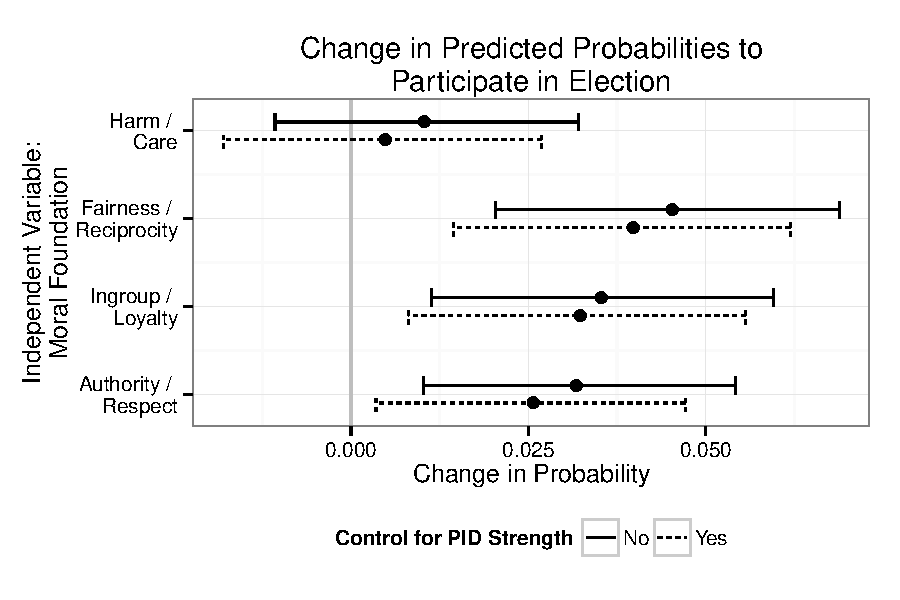
\includegraphics[scale=.9]{../calc/fig/fig5turnout.pdf}
\caption{Difference in predicted probabilities to participate in different forms of political action when the aggregated similarity score is increased from its minimum (no overlap between dictionary and response) by one standard deviation, holding all other control variables constant at their respective means (along with 95\% confidence intervals). Positive values indicate that respondents who mentioned the respective foundation are more likely to participate, and vice versa. Estimates are based on a logit models including the normalized sum of similaritiy scores for each foundation and dotted lines indicate estimates while additionally controlling for the strength of party identification. Additional plot including 2008 data is shown in the appendix, Figure~\ref{fig:appD9turnout}, and full model results are displayed in Table~\ref{tab:m5turnout}.}\label{fig:5turnout}
\end{figure}

Moral reasoning about political attitudes has a positive effect on the predicted probabilities of participating in each from of political action. For example, if the aggregate similarity score is increased from its minimum (i.e. no moral reasoning at all) by one standard deviation, probability of turning out to vote is increased by almost 2 percentage points, holding all other variables constant at their respective means. Note that the estimates are based on models that take into account the length of individual responses. Furthermore, all effects stay significant and are only reduced marginally after controlling for the strength of individual party identification.

These effects might not seem large, but bear in mind that the independent variable consists of a measure of emphasis of moral considerations in open-ended questions. The fact that we can recover consistent and statistically significant effects on political participation in such a context (even after controlling for strength of party identification and the length of individual responses) is therefore quite meaningful.

Overall then, the analyses indicate that moral reasoning is positively associated with political engagement. That said, the analyses presented here are not sufficient to make a strong causal claim about the direction of this relationship. Yet, the results suggest that moral reasoning (as measured by open-ended survey responses) is powerfully related to different forms of political participation and engagement.


\section{Conclusion}

The goal of this paper was to investigate whether the ideological differences in the emphasis of moral foundations manifests itself in individual reasoning about political actors. The analyses of open-ended survey responses can provide important insights beyond previous research because it allows us to evaluate whether citizens make references to moral considerations in a political context that does not induce an explicit connection to morality. In contrast to previous accounts of Moral Foundations theory, I argue that the reliance on moral reasoning as such is moderated by political knowledge, media exposure, and political discussions. The emphasis of specific moral foundations, in turn, was expected to influence important political outcomes such as candidate evaluations and voting behavior. Furthermore, general tendencies to take into account moral considerations should affect different measures of political participation.

The empirical evidence discussed in this paper extends and qualifies previous research on moral foundations and ideology. The first hypothesis, which predicted systematic patterns in the emphasis on moral considerations among liberals and conservatives, was supported for three out of four foundations. Liberals are more likely to mention considerations related to harm/care and fairness/reciprocity when discussing their political preferences, whereas conservatives are more likely to emphasize the moral foundation of ingroup/loyalty. Evidence for the authority/respect dimension was tentatively consistent with our expectations, but not statistically significant.

According to the second hypothesis, it was expected that individuals show heterogeneity in terms of their tendency to rely on moral reasoning. The results indicated that political knowledge, discussions, as well as media consumption increase the reliance on moral considerations. Thus, the evidence suggests that moral reasoning is part of a broader political learning process. At least in some cases, this learning process appears to imply an increased differentiation between liberals and conservatives in terms of the focus on specific foundations as described by Moral Foundations Theory.

The last part of the analyses focused on the political relevance of moral reasoning as conceptualized by open-ended survey responses. The results here revealed consistent relationships between individual moral foundations and political preferences and voting behavior. Furthermore, general moral references consistently increase the likelihood of participating in political action. As such, moral reasoning measured using open-ended survey responses is a politically meaningful and influential concept.

The contributions of this paper are therefore twofold. This study adds to the existing literature on moral foundations by providing new insights into the mechanisms underlying its relationship with ideology. From a general methodological perspective, the paper emphasizes the potential benefits of incorporating open-ended survey responses in research focusing on the determinants and structure of ideology and political reasoning. The paper shows that one can directly assess moral reasoning in surveys that do not contain the MFQ or related measures, simply by relying on open-ended survey responses.

However, it should be noted that many of the relationships discussed in the paper could not be recovered in a replication using data from the 2008 ANES. While the basic patterns persist, many effects in 2008 fail to reach statistical significance. This issue can partly be explained by the fact that the open-ended responses in 2008 were recorded by some interviewers as indirect summaries rather than direct verbatim responses. As such, the open-ended survey data for 2012 is better suited to identify moral references through the respondent's open-ended responses.

The results presented here provide several directions for future research. The fact that purity/sanctity was almost never mentioned as well as the inconsistent effect of ideology on the authority/respect dimension can be attributed to the fact that the moral foundations dictionary was originally used for the analyses of sermons. Accordingly, subsequent analyses could revise the dictionary in order to make it more applicable for the analyses of survey responses. An alternative approach to the analysis of open-ended survey responses could be the implementation of structural topic models as described by \citet{roberts2014structural}: instead of using explicit word lists to identify moral reasoning, it would possible to identify specific topics in open-ended responses that are consistent with the moral foundations described by \citet{haidt2008moral} \citep[see also][]{lin2008joint}.

One important issue that remains unresolved is the question of causality. \citet{graham2009liberals} rightfully stated that the causal nature of the relationship between moral foundations and ideology is not yet established. Their study did not settle whether individuals first identify as liberal or conservative and then adapt their respective moral judgments, or whether moral considerations shape and structure subsequent ideological thinking itself. Recent research focusing on elite influences on moral reasoning suggests that elite rhetoric plays an important role in shaping individual moral judgment \citep[see for example][]{clifford2013words,clifford2015concerns}. However, directly examining the underlying causal mechanism requires additional research where moral reasoning is manipulated experimentally.

It would also be worth investigating whether the patterns regarding moral reasoning change over longer periods of time using this method in order to further establish the context-specific nature of moral reasoning. At this time, however, full-text open-ended survey responses are not available in the ANES prior to 2008.

Overall, the analyses of open-ended survey responses can provide important and valuable insights in the context of moral foundations and the individual underpinnings of political ideology. Utilizing available responses to open-ended survey questions provides a useful and still largely neglected data source to investigate political reasoning.

% Broader idea, we wouldn't be constrained to the dictionaries, we could also just use sample texts? think about this idea a bit more

% Argument for conclusion: politics is social, we should look at language to understand interpresonal influence etc. 
% we can better understand polarization etc. if we directly look at moral reasoning and therefore at the tendency of individuals to rely on moral considerations when talking about politics.


\clearpage
\bibliographystyle{/data/Copy/1-src/lit/apsr2006}
\bibliography{/data/Copy/1-src/lit/Literature}

\clearpage
\footnotesize\singlespacing
\appendices
\appendixpage
\renewcommand\thesubsection{\Roman{subsection}}
\begin{flushleft}
Kraft, Patrick W. 2016.\\``Moral Foundations of Political Reasoning. Investigating the Moral Underpinnings of Political Judgment.''

\startcontents[sections]
\printcontents[sections]{l}{1}{\setcounter{tocdepth}{2}}
\clearpage

\section{Moral Foundations Dictionary}\label{app:dict}
\renewcommand\thefigure{\thesection.\arabic{figure}}
\renewcommand\thetable{\thesection.\arabic{table}}
\setcounter{figure}{0}
\setcounter{table}{0}

\textit{Sources:}\\
\citet{graham2009liberals}, as well as \url{http://www.moralfoundations.org/}
\vspace{.5cm}

\textit{Note:}\\
Words with (*) indicate that the word stem rather than the exact word was matched in the open-ended survey responses.
\vspace{.5cm}

\textbf{Harm:}\\
safe*, peace*, compassion*, empath*, sympath*, care, caring, protect*, shield, shelter, amity, secur*, benefit*, defen*, guard*, preserve, harm*, suffer*, war, wars, warl*, warring, fight*, violen*, hurt*, kill, kills, killer*, killed, killing, endanger*, cruel*, brutal*, abuse*, damag*, ruin*, ravage, detriment*, crush*, attack*, annihilate*, destroy, stomp, abandon*, spurn, impair, exploit, exploits, exploited, exploiting, wound*
\vspace{.5cm}

\textbf{Fairness:}\\
fair, fairly, fairness, fair*, fairmind*, fairplay, equal*, justice, justness, justifi*, reciproc*, impartial*, egalitar*, rights, equity, evenness, equivalent, unbias*, tolerant, equable, balance*, homologous, unprejudice*, reasonable, constant, honest*, unfair*, unequal*, bias*, unjust*, injust*, bigot*, discriminat*, disproportion*, inequitable, prejud*, dishonest, unscrupulous, dissociate, preference, favoritism, segregat*, exclusion, exclud*
\vspace{.5cm}

\textbf{Ingroup:}\\
together, nation*, homeland*, family, families, familial, group, loyal*, patriot*, communal, commune*, communit*, communis*, comrad*, cadre, collectiv*, joint, unison, unite*, fellow*, guild, solidarity, devot*, member, cliqu*, cohort, ally, insider, foreign*, enem*, betray*, treason*, traitor*, treacher*, disloyal*, individual*, apostasy, apostate, deserted, deserter*, deserting, deceiv*, jilt*, imposter, miscreant, spy, sequester, renegade, terroris*, immigra*
\vspace{.5cm}

\textbf{Authority:}\\
obey*, obedien*, duty, law, lawful*, legal*, duti*, honor*, respect, respectful*, respected, respects, order*, father*, mother, motherl*, mothering, mothers, tradition*, hierarch*, authorit*, permit, permission, status*, rank*, leader*, class, bourgeoisie, caste*, position, complian*, command, supremacy, control, submi*, allegian*, serve, abide, defere*, defer, revere*, venerat*, comply, defian*, rebel*, dissent*, subver*, disrespect*, disobe*, sediti*, agitat*, insubordinat*, illegal*, lawless*, insurgent, mutinous, defy*, dissident, unfaithful, alienate, defector, heretic*, nonconformist, oppose, protest, refuse, denounce, remonstrate, riot*, obstruct
\vspace{.5cm}

\textbf{Purity:}\\
piety, pious, purity, pure*, clean*, steril*, sacred*, chast*, holy, holiness, saint*, wholesome*, celiba*, abstention, virgin, virgins, virginity, virginal, austerity, integrity, modesty, abstinen*, abstemiousness, upright, limpid, unadulterated, maiden, virtuous, refined, intemperate, decen*, immaculate, innocent, pristine, humble, disgust*, deprav*, disease*, unclean*, contagio*, indecen*, sin, sinful*, sinner*, sins, sinned, sinning, slut*, whore, dirt*, impiety, impious, profan*, gross, repuls*, sick*, promiscu*, lewd*, adulter*, debauche*, defile*, tramp, prostitut*, unchaste, wanton, profligate, filth*, trashy, obscen*, lax, taint*, stain*, tarnish*, debase*, desecrat*, wicked*, blemish, exploitat*, pervert, wretched*
\vspace{.5cm}

%\textbf{General:}\\
%righteous*, moral*, ethic*, value*, upstanding, good, goodness, principle*, blameless, exemplary, lesson, canon, doctrine, noble, worth*, ideal*, praiseworthy, commendable, character, proper, laudable, correct, wrong*, evil, immoral*, bad, offend*, offensive*, transgress*, honest*, lawful*, legal*, piety, pious, wholesome*, integrity, upright, decen*, indecen*, wicked*, wretched*

\end{flushleft}

\clearpage
\section{Overview Open-Ended Responses}\label{app:oview}
\renewcommand\thefigure{\thesection.\arabic{figure}}
\renewcommand\thetable{\thesection.\arabic{table}}
\setcounter{figure}{0}
\setcounter{table}{0}

% latex table generated in R 3.2.3 by xtable 1.7-4 package
% Tue Jan 19 19:37:46 2016
\begin{table}[ht]
\centering
\begin{tabular}{lcc}
  \hline
 & N & Percent \\ 
  \hline
Spanish Interview (2008) & 94 & 4.05 \\ 
  Spanish Interview (2012) & 228 & 3.86 \\ 
  No Responses (Overall, 2008) & 158 & 7.09 \\ 
  No Responses (Overall, 2012) & 392 & 6.89 \\ 
  No Responses (Candidate Evaluations, 2008) & 328 & 14.13 \\ 
  No Responses (Candidate Evaluations, 2012) & 761 & 12.87 \\ 
  No Responses (Party Evaluations, 2008) & 584 & 25.15 \\ 
  No Responses (Party Evaluations, 2012) & 1503 & 25.41 \\ 
   \hline
\end{tabular}
\caption{Missing open-ended responses} 
\label{tab:appB1mis}
\end{table}


\begin{figure}[h]\centering
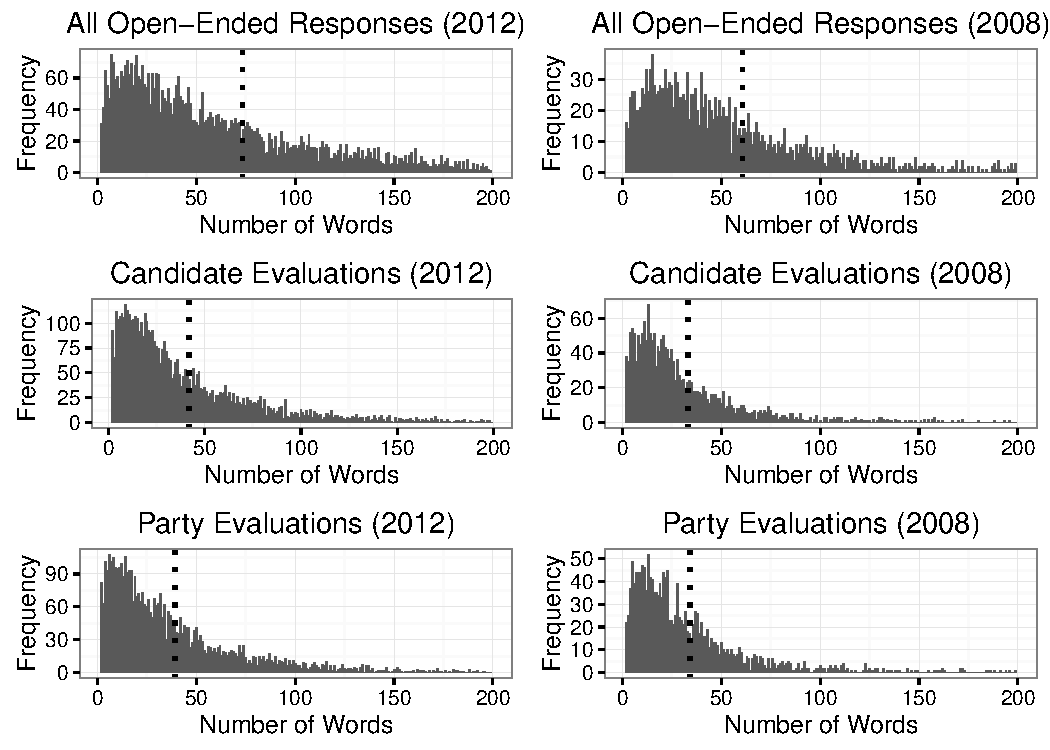
\includegraphics[scale=.7]{../calc/fig/appB2num.pdf}
\caption{Histograms displaying the distribution of individual response lengths in number of words for each respective item category. Dotted lines indicate the average response length.}\label{fig:appB2num}
\end{figure}

\clearpage
\section{Description of Moral Reasoning Measure}\label{app:measure}

This part of the appendix contains a detailed description of the measure of moral reasoning used throughout the paper. It is based on open-ended survey responses as well as the moral dictionary proposed by \citet{graham2009liberals}. All techniques described here are adapted from common approaches in quantitative text analysis and information retrieval \citep[see for exampe][for an introduction and from which much of the notation in this part of the appendix is adapted]{manning2008introduction}.

As a first step, each individual response as well as the moral foundations dictionaries are converted into a \textit{document-term matrix}. Each row in the document-term matrix represents one document (i.e. the collection of open-ended responses for one individual, or the dictionary for a single moral foundation, respectively). Each column represents a term that is contained in the complete vocabulary of the corpus (i.e. all columns encompass the set of unique words contained in all documents). Each element in the matrix indicates the number of times the term is included in the respective document. As such, the matrix consists of raw frequencies of term $t$ in document $d$ (often denoted by tf$_{t,d}$).

However, in the context of information retrieval that aims at matching string queries with most relevant matches out of a set of documents, term frequencies are usually weighted by the \textit{inverse document frequency} in order to account for the fact that some terms have more discriminative power than others. The underlying logic is that a word that appears in almost all of the documents should be less decisive in affecting the similarity between the query and the document than a term that only appears in a selection of documents. The inverse document frequency is usually defined as
\begin{equation}
\text{idf}_t = \log \tfrac{N}{\text{df}_t},
\end{equation}
where $N$ is the total number of documents in the corpus, and $df_t$ denotes the number of documents in which term $t$ occurs. The tf-idf score of term $t$ in document $d$ is then computed as
\begin{equation}
\text{tf-idf}_{t,d} = \text{tf}_{t,d} * \text{idf}_t.
\end{equation}
Raw term frequencies are therefore weighted by the inverse of the term's document frequency, which leads to increased (decreased) values if a term is only included in few (many) documents. We can now represent each moral dictionary and response as a vector of tf-idf scores for each term. For convenience, let $w_{t,d}$ be the tf-idf score for term $t$ in the dictionary and document $d$ (which could be a moral dictionary or an open-ended response). Then,
\begin{align}
\vec{m}_j &= \left(w_{1,j},w_{2,j},\cdots, w_{T,j}\right) \\
\vec{r}_n &= \left(w_{1,n},w_{2,n},\cdots, w_{T,n}\right),
\end{align}
where $\vec{m}_j$ denotes the moral dictionary for foundation $j\in\{1,\cdots,J\}$, $\vec{r}_n$ denotes the open-ended responses of individual $n\in\{1,\cdots,N\}$, and $T$ denotes the total number of unique terms in the entire text corpus. This representation of documents and queries (or in our case dictionaries) is usually described as the \textit{vector space model} for representing the corpus.

Each moral dictionary and open-ended response is now represented as a vector of length $T$. A common measure of relevance, for example of a document ($\vec{r}_n$) for a keyword search query (in our case $\vec{m}_j$), is the cosine similarity:
\begin{equation}
\cos\theta_{j,n}=\dfrac{\vec{m}(j)\cdotp\vec{r}(n)}{|\vec{m}(j)||\vec{r}(n)|},
\end{equation}
where $\vec{m}(j)\cdotp\vec{r}(n)$ is the dot-product of the dictionary and the response, and $|\vec{m}(j)||\vec{r}(n)|$ is the product of the Euclidean norm of both vectors. $\theta_{j,n}$ can therefore be understood as the angle between the vector space representation of the moral foundation dictionary $j$ and the open-ended response of individual $n$. The cosine score is 1 if the relative frequency of words used by the respondent overlap completely with the terms in the dictionary (not that this holds irrespective of the length of the response), and 0 if there is no overlap.


\clearpage
\section{Additional Descriptive Plots}\label{app:desc}
\renewcommand\thefigure{\thesection.\arabic{figure}}
\renewcommand\thetable{\thesection.\arabic{table}}
\setcounter{figure}{0}
\setcounter{table}{0}

\begin{figure}[h]
  \centering
  \caption{Weighted proportion of Respondents mentioning each of the moral foundations in any of their open-ended responses, along with 95\% confidence intervals.}
  \begin{subfigure}[t]{0.49\textwidth}
    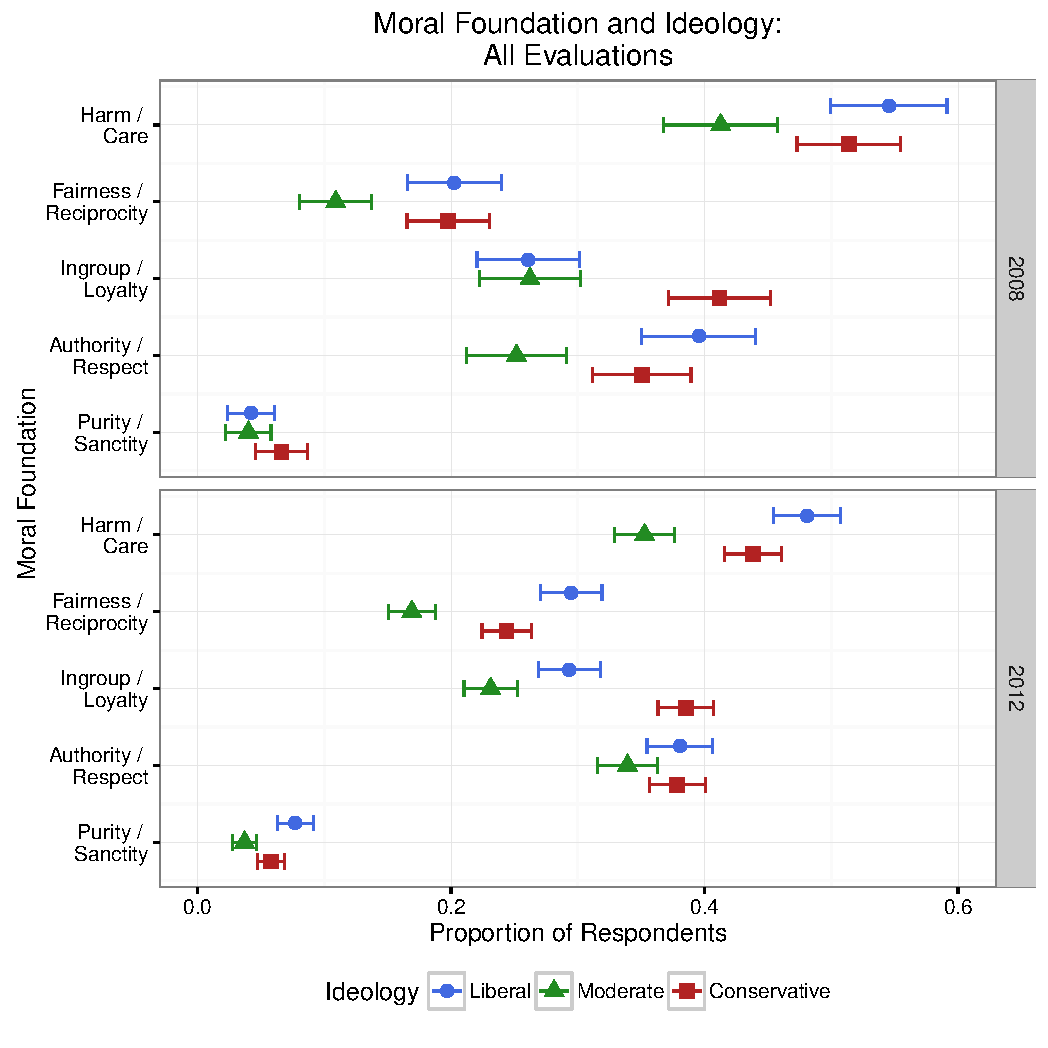
\includegraphics[scale=.4]{../calc/fig/appC1prop.pdf}
\caption{Proportions based on all open-ended responses}\label{fig:appC1prop}
  \end{subfigure}
  \begin{subfigure}[t]{0.49\textwidth}
    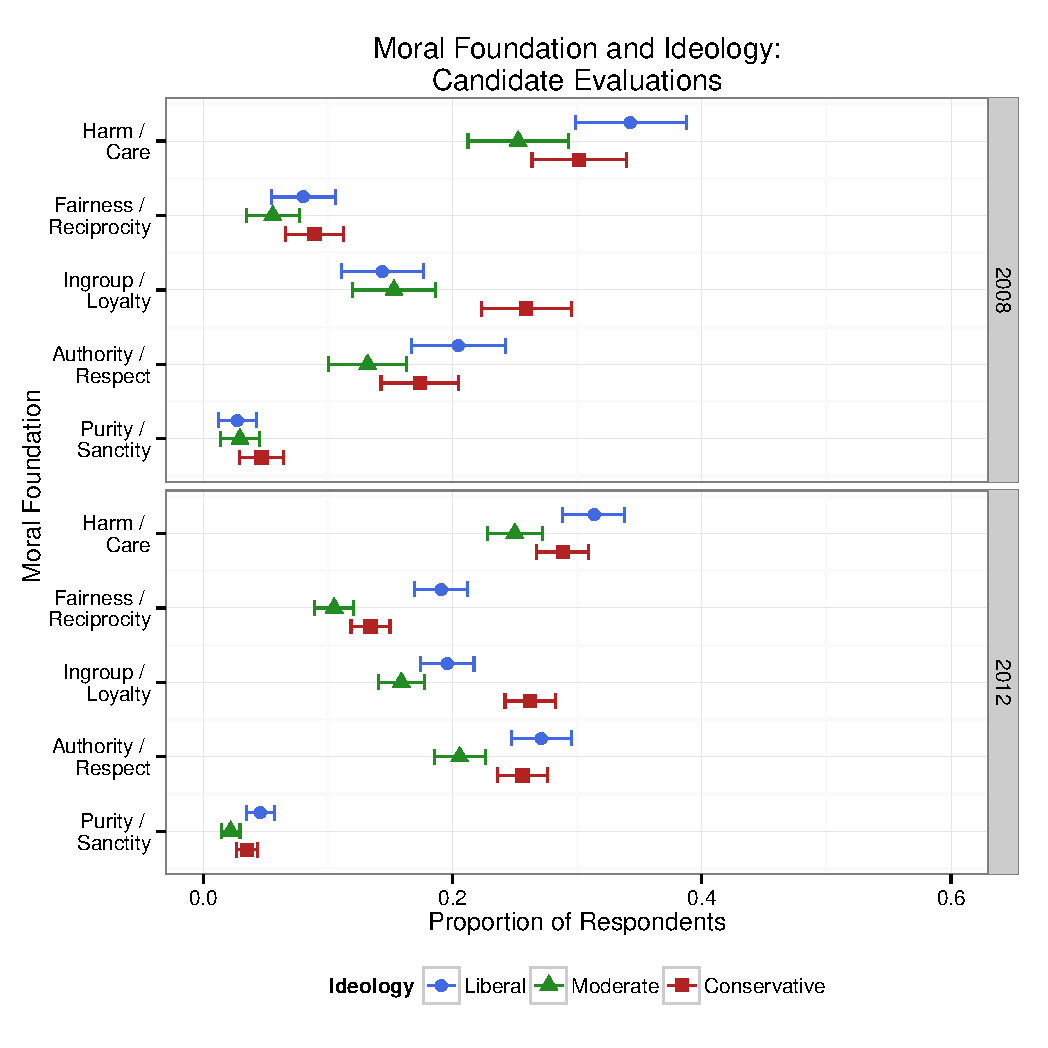
\includegraphics[scale=.4]{../calc/fig/appC2cand.pdf}
\caption{Proportions based on candidate evaluations}\label{fig:appC2cand}
  \end{subfigure}
  \begin{subfigure}[t]{0.49\textwidth}
    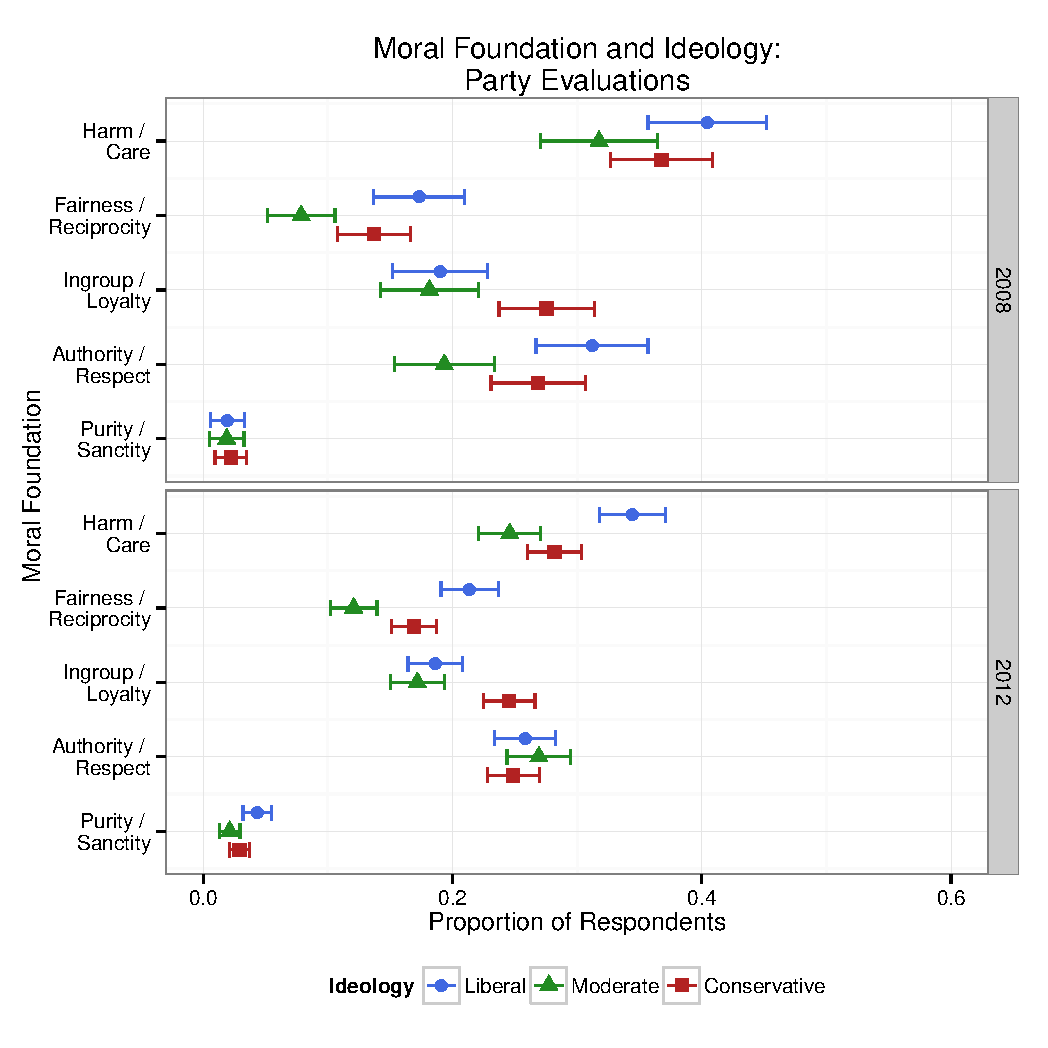
\includegraphics[scale=.4]{../calc/fig/appC3party.pdf}
\caption{Proportions based on party evaluations}\label{fig:appC3party}
  \end{subfigure}
\end{figure}


\clearpage
\section{Alternative Model Specifications and Robustness Checks}\label{app:robust}
\renewcommand\thefigure{\thesection.\arabic{figure}}
\renewcommand\thetable{\thesection.\arabic{table}}
\setcounter{figure}{0}
\setcounter{table}{0}


\subsection{Ideological differences in moral reasoning including 2008 ANES data}

\begin{figure}[h]
  \centering
  \caption{Difference in predicted probabilities to reference each moral foundation between liberals and conservatives, holding all other control variables at their respective means (along with 95\% confidence intervals). Positive values indicate that conservatives are more likely to reference the respective moral foundations than liberals, and vice versa. Estimates are based on seemingly unrelated regressions for each foundation's similarity score.}
  \begin{subfigure}[t]{0.49\textwidth}
    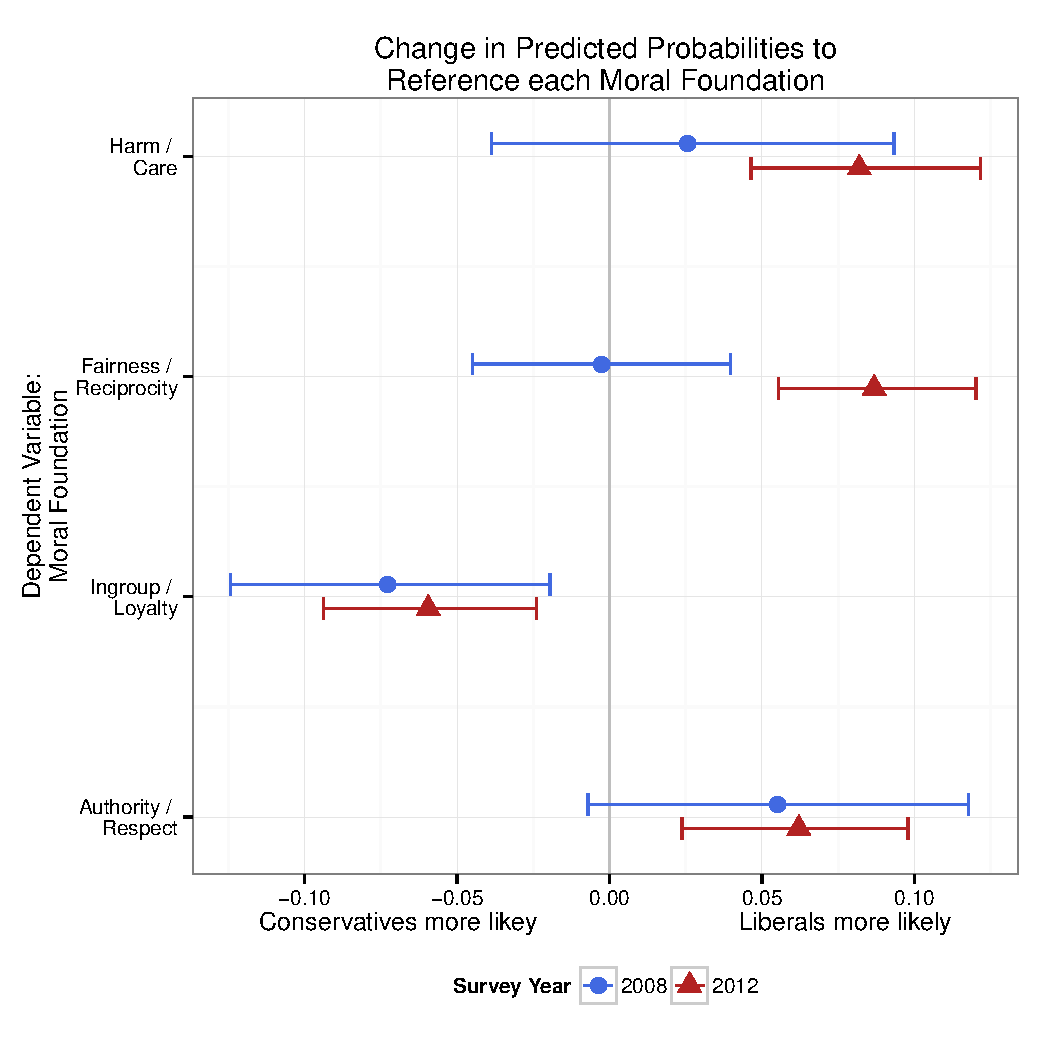
\includegraphics[scale=.4]{../calc/fig/appD1ideol.pdf}
    \caption{Basic models including data from 2008 ANES. Full model results are reported in Table \ref{tab:m2ideol}.}\label{fig:appD1ideol}
  \end{subfigure}
\end{figure}

\clearpage
\subsection{Determinants of moral reasoning including 2008 ANES data}

\begin{figure}[h]
  \centering
  \caption{Models predicting probabilities to reference any moral foundation including 2008 ANES data.}
  \begin{subfigure}[t]{0.49\textwidth}
    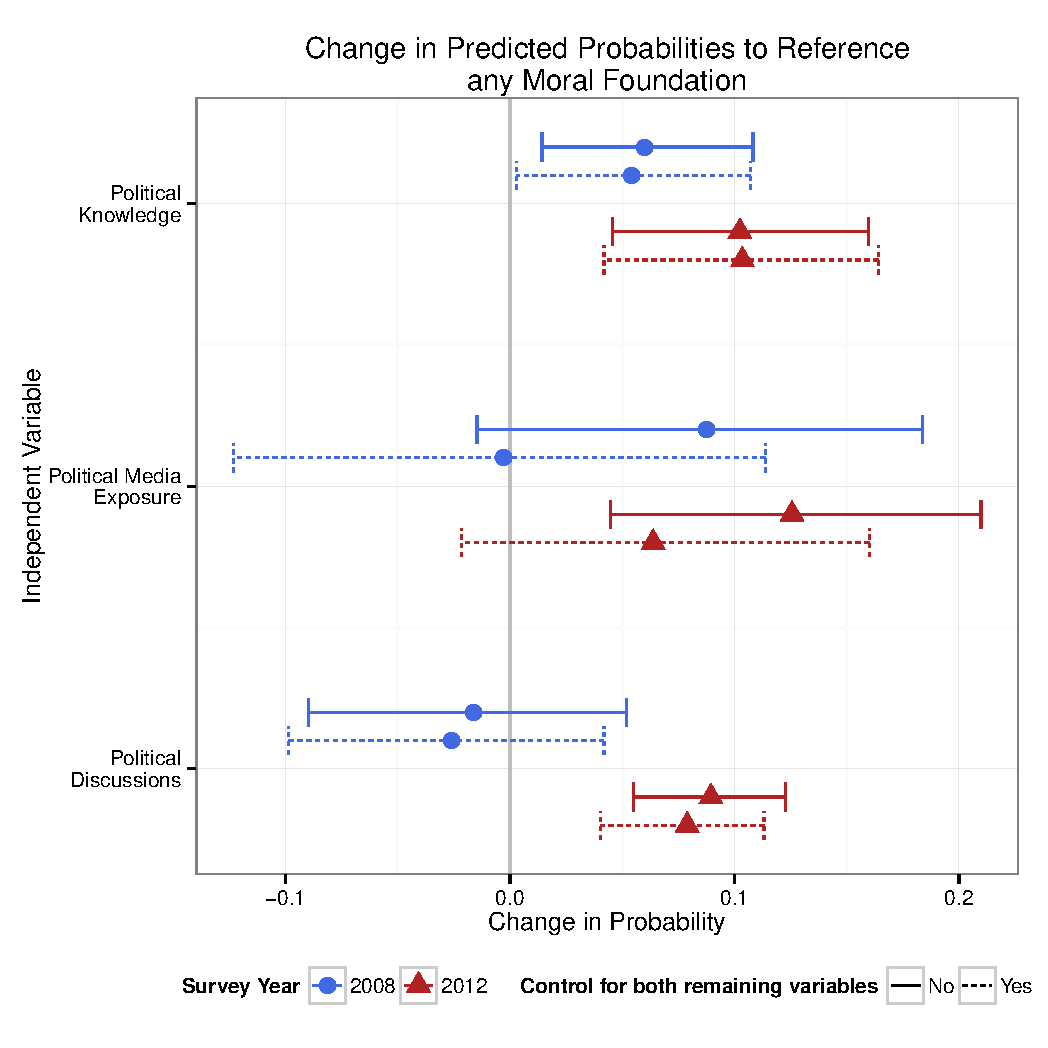
\includegraphics[scale=.4]{../calc/fig/appD7learn.pdf}
    \caption{Change in predicted emphasis on any moral foundation depending on political knowledge, media exposure, and frequency of political discussions. The plot shows the difference in the expected values if each of the independent variables is increased from its minimum to its maximum value holding all other variables constant at their respective means (along with 95\% confidence intervals). Positive values indicate higher probabilities of referencing any moral foundation. Estimates are based on logit models and dotted lines indicate estimates while controlling for both remaining variables. Full model results are reported in Table \ref{tab:m3learn}.}\label{fig:appD7learn}
  \end{subfigure}
  \begin{subfigure}[t]{0.49\textwidth}
    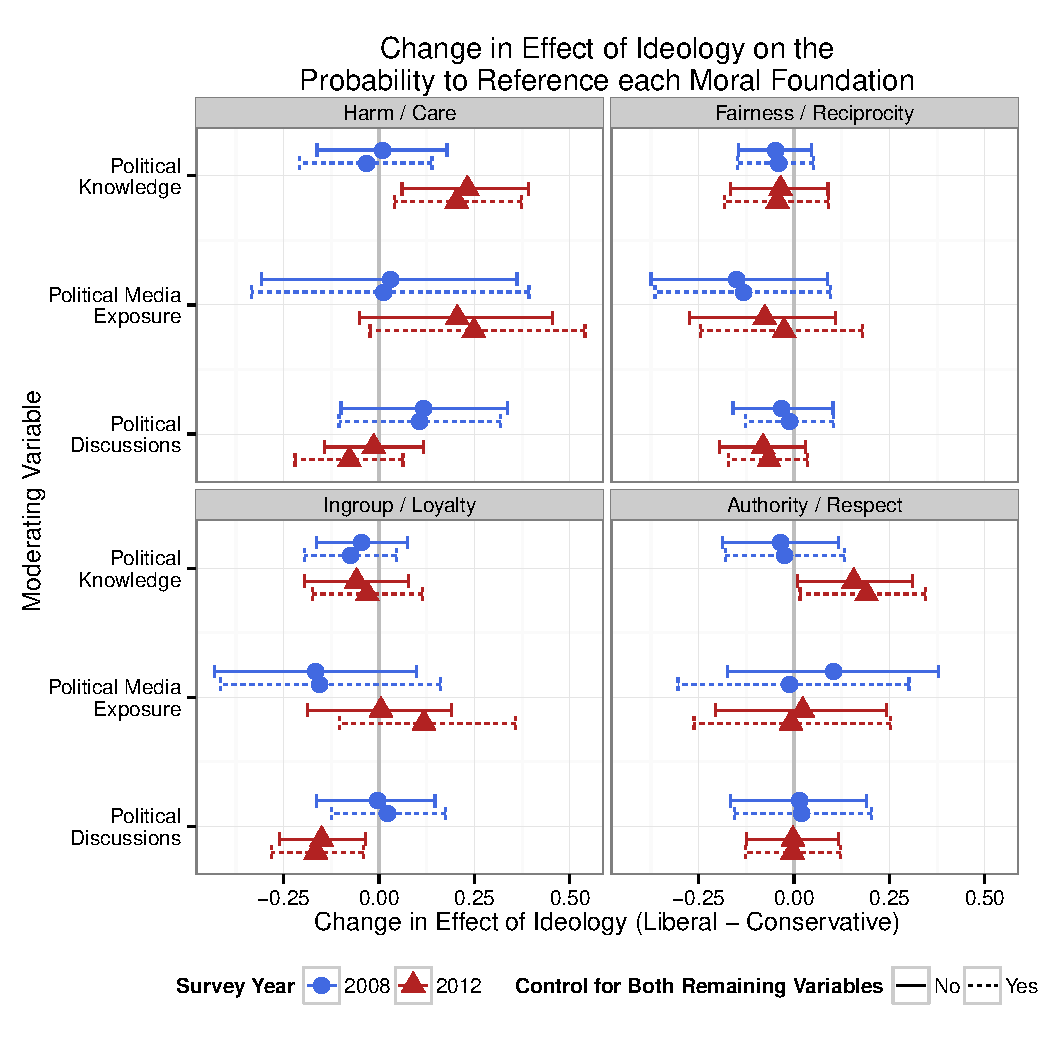
\includegraphics[scale=.4]{../calc/fig/appD8ideolearn.pdf}
    \caption{Change in effect of ideology on predicted emphasis on any moral foundation moderated by political knowledge, media exposure, and frequency of political discussions (difference-in-difference). The plot shows how the difference in predicted probabilities to reference each moral foundation between liberals and conservatives changes if each of the independent variables is increased from its minimum to its maximum value holding all other variables constant at their respective means (along with 95\% confidence intervals). Positive values indicate that liberals are more likely to mention a specific moral foundation if they score high on the moderating variable (knowledge, exposure, or discussions), and vice versa. Estimates are based on individual logit models for each foundation and dotted lines indicate estimates while controlling for both remaining variables. Full model results are reported in Tables \ref{tab:m4ideolearn2012a} to \ref{tab:m4ideolearn2008b}.}\label{fig:appD8ideolearn}
  \end{subfigure}
\end{figure}


\clearpage
\subsection{Consequences and political relevance of moral reasoning including 2008 ANES data}

\begin{figure}[h]
  \centering
  \caption{Models predicting feeling thermometer differentials and vote choice based on moral reasoning including 2008 ANES data.}
  \begin{subfigure}[t]{0.49\textwidth}
    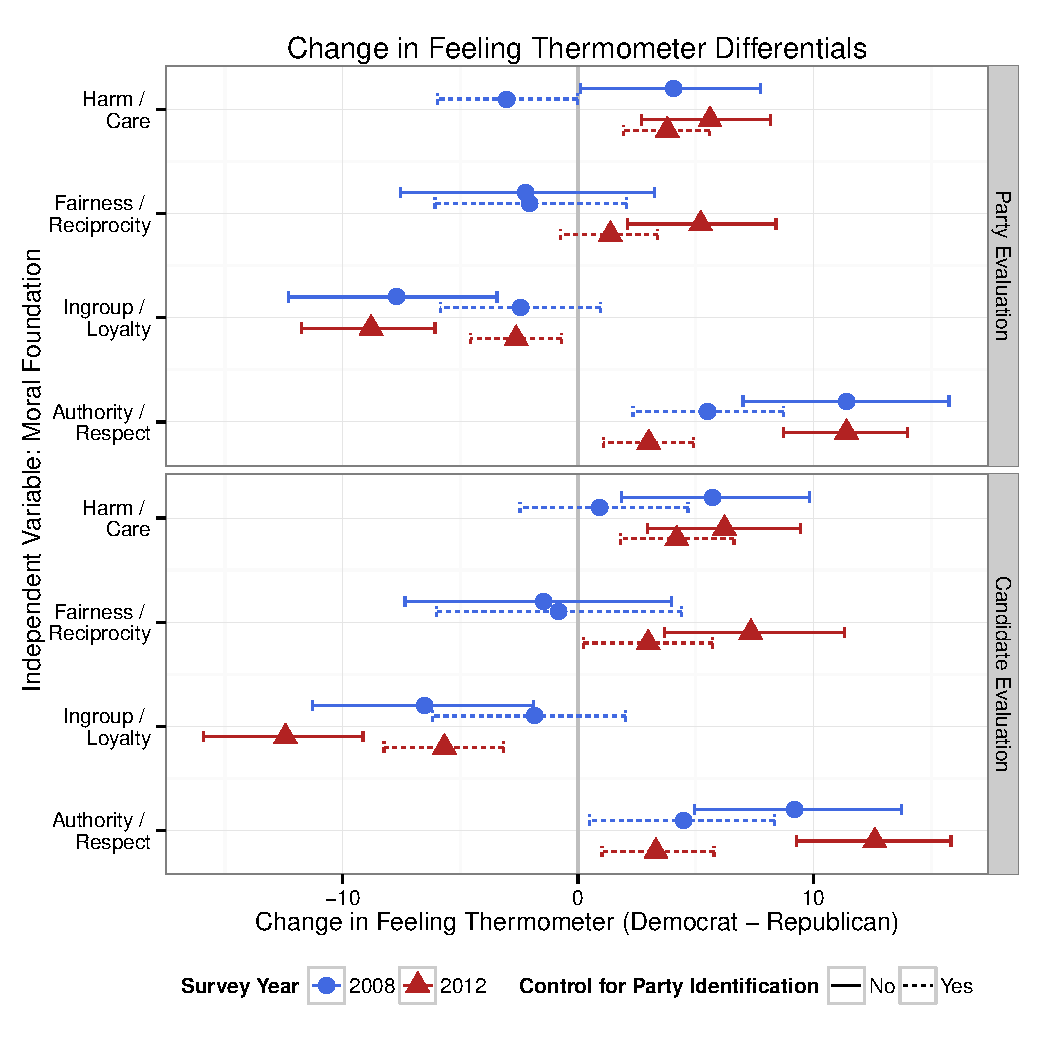
\includegraphics[scale=.4]{../calc/fig/appD11feel.pdf}
    \caption{Change in predicted feeling thermometer differential between respondents who mentioned each moral foundation or not, holding all other control variables constant at their respective means (along with 95\% confidence intervals). Positive values indicate that respondents who mentioned the respective foundation evaluated the Democratic candidate/party more favorably than the Republican candidate/party, and vice versa. Estimates are based on a single OLS model (using robust standard errors) including dichotomous indicators for each foundation and dotted lines indicate estimates while additionally controlling for party identification. Full model results are reported in Table \ref{tab:m7feel}.}\label{fig:appD11feel}
  \end{subfigure}
  \begin{subfigure}[t]{0.49\textwidth}
    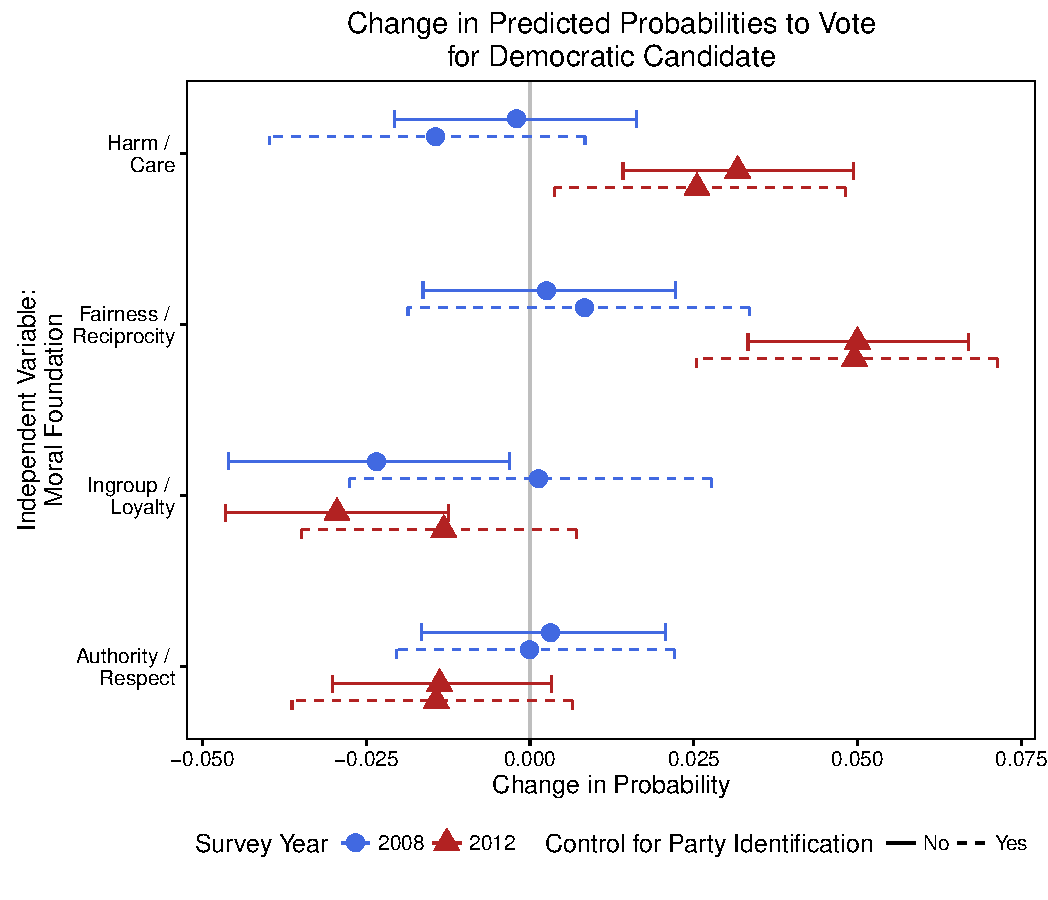
\includegraphics[scale=.4]{../calc/fig/appD12vote.pdf}
    \caption{Difference in predicted probabilities to vote for Democratic candidate between respondents who mentioned each moral foundation or not, holding all other control variables constant at their respective means (along with 95\% confidence intervals). Positive values indicate that respondents who mentioned the respective foundation are more likely to vote for the Democratic candidate, and vice versa. Estimates are based on a single logit model including dichotomous indicators for each foundation and dotted lines indicate estimates while additionally controlling for party identification. Full model results are reported in Table \ref{tab:m8vote}.}\label{fig:appD12vote}
  \end{subfigure}
\end{figure}

\begin{figure}[t]
  \centering
    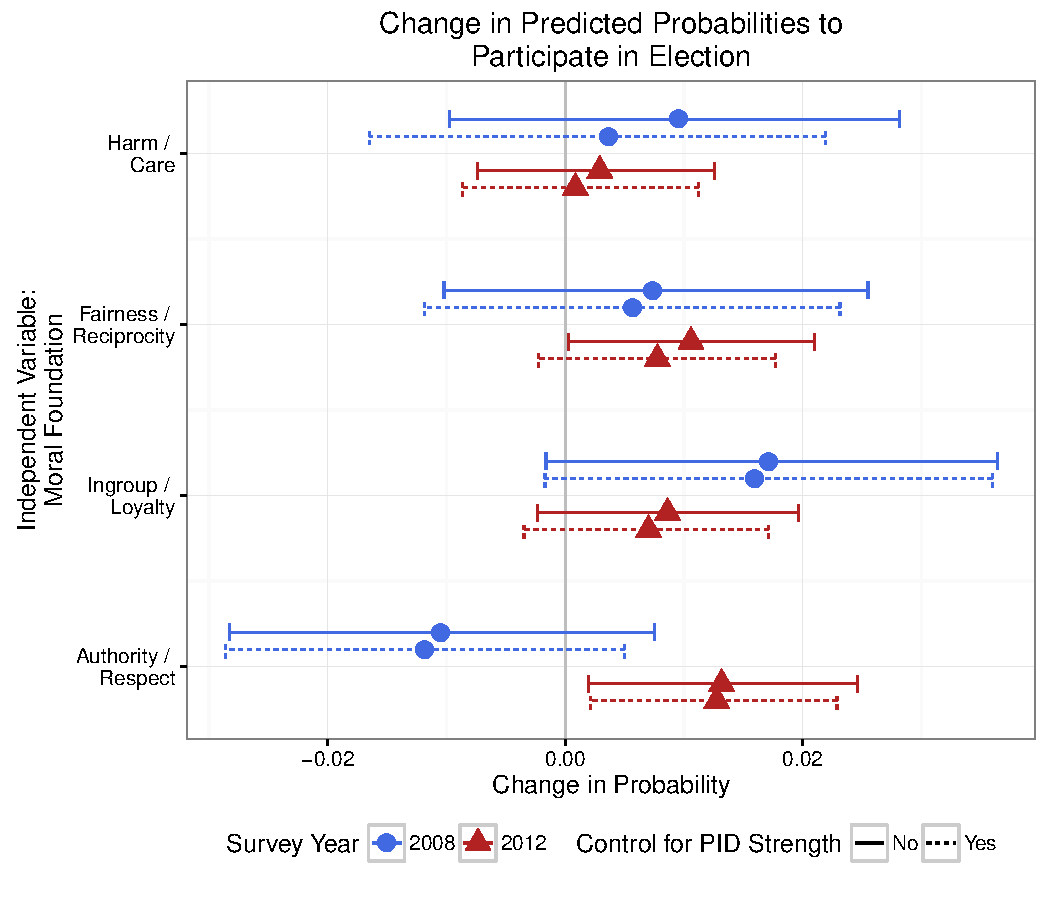
\includegraphics[scale=.4]{../calc/fig/appD9turnout.pdf}
    \caption{Models predicting turnout based on moral reasoning including 2008 ANES data. Difference in predicted probabilities to participate in election between respondents who mentioned each moral foundation or not, holding all other control variables constant at their respective means (along with 95\% confidence intervals). Positive values indicate that respondents who mentioned the respective foundation are more likely to participate in the election, and vice versa. Estimates are based on a single logit model including dichotomous indicators for each foundation and dotted lines indicate estimates while additionally controlling for the strength of party identification. Full model results are reported in Table \ref{tab:m5turnout}}\label{fig:appD9turnout}
\end{figure}


\clearpage
\section{Tables of Model Estimates}\label{app:tables}
\renewcommand\thefigure{\thesection.\arabic{figure}}
\renewcommand\thetable{\thesection.\arabic{table}}
\setcounter{figure}{0}
\setcounter{table}{0}


\subsection{Ideological differences in moral reasoning including 2008 ANES data}


% Table created by stargazer v.5.2 by Marek Hlavac, Harvard University. E-mail: hlavac at fas.harvard.edu
% Date and time: Wed, Jan 20, 2016 - 12:21:34 PM
% Requires LaTeX packages: dcolumn 
\begin{table}[ht] \centering 
  \caption{Logit Models Predicting References to four Moral Foundations using Ideology} 
  \label{tab:m2ideol} 
\tiny 
\begin{tabular}{@{\extracolsep{-15pt}}lD{.}{.}{-3} D{.}{.}{-3} D{.}{.}{-3} D{.}{.}{-3} D{.}{.}{-3} D{.}{.}{-3} D{.}{.}{-3} D{.}{.}{-3} } 
\\[-1.8ex]\hline 
\hline \\[-1.8ex] 
 & \multicolumn{8}{c}{\textit{Dependent variable:}} \\ 
\cline{2-9} 
\\[-1.8ex] & \multicolumn{2}{c}{Harm / Care} & \multicolumn{2}{c}{Fairness / Reciprocity} & \multicolumn{2}{c}{Ingroup / Loyalty} & \multicolumn{2}{c}{Authority / Respect} \\ 
 & \multicolumn{1}{c}{2012} & \multicolumn{1}{c}{2008} & \multicolumn{1}{c}{2012} & \multicolumn{1}{c}{2008} & \multicolumn{1}{c}{2012} & \multicolumn{1}{c}{2008} & \multicolumn{1}{c}{2012} & \multicolumn{1}{c}{2008} \\ 
\hline \\[-1.8ex] 
 Conservative & -0.340^{***} & -0.103 & -0.492^{***} & 0.019 & 0.298^{***} & 0.475^{***} & -0.272^{***} & -0.270^{*} \\ 
  & (0.083) & (0.148) & (0.092) & (0.191) & (0.090) & (0.171) & (0.085) & (0.152) \\ 
  Moderate & -0.338^{***} & -0.131 & -0.518^{***} & -0.273 & -0.026 & 0.367^{**} & -0.133 & -0.375^{**} \\ 
  & (0.084) & (0.150) & (0.094) & (0.209) & (0.095) & (0.178) & (0.085) & (0.159) \\ 
  Church Attendance & -0.016 & -0.039 & -0.0003 & -0.016 & 0.042^{**} & -0.012 & -0.030 & 0.052 \\ 
  & (0.019) & (0.035) & (0.022) & (0.046) & (0.021) & (0.039) & (0.020) & (0.036) \\ 
  Education (College Degree) & -0.017 & 0.139 & 0.322^{***} & 0.225 & 0.394^{***} & 0.554^{***} & 0.211^{***} & 0.321^{**} \\ 
  & (0.070) & (0.124) & (0.076) & (0.173) & (0.073) & (0.148) & (0.070) & (0.134) \\ 
  Age & -0.004^{*} & -0.015^{***} & 0.004^{*} & 0.011^{**} & -0.002 & -0.009^{**} & 0.007^{***} & -0.004 \\ 
  & (0.002) & (0.004) & (0.002) & (0.005) & (0.002) & (0.004) & (0.002) & (0.004) \\ 
  Sex (Female) & 0.200^{***} & 0.017 & 0.110 & 0.028 & -0.128^{*} & -0.432^{***} & -0.083 & -0.205^{*} \\ 
  & (0.066) & (0.118) & (0.074) & (0.157) & (0.072) & (0.134) & (0.067) & (0.124) \\ 
  Race (African American) & -0.017 & -0.066 & -0.103 & -0.042 & -0.189^{*} & -0.253 & 0.378^{***} & -0.081 \\ 
  & (0.091) & (0.150) & (0.105) & (0.207) & (0.103) & (0.180) & (0.091) & (0.160) \\ 
  Number of Words & 0.014^{***} & 0.017^{***} & 0.009^{***} & 0.008^{***} & 0.013^{***} & 0.015^{***} & 0.013^{***} & 0.011^{***} \\ 
  & (0.001) & (0.001) & (0.0005) & (0.001) & (0.001) & (0.001) & (0.001) & (0.001) \\ 
  Constant & -0.978^{***} & -0.614^{***} & -1.909^{***} & -3.026^{***} & -2.004^{***} & -2.071^{***} & -1.727^{***} & -1.366^{***} \\ 
  & (0.125) & (0.227) & (0.142) & (0.321) & (0.140) & (0.270) & (0.131) & (0.241) \\ 
 \hline \\[-1.8ex] 
Observations & \multicolumn{1}{c}{4,691} & \multicolumn{1}{c}{1,468} & \multicolumn{1}{c}{4,691} & \multicolumn{1}{c}{1,468} & \multicolumn{1}{c}{4,691} & \multicolumn{1}{c}{1,468} & \multicolumn{1}{c}{4,691} & \multicolumn{1}{c}{1,468} \\ 
Log Likelihood & \multicolumn{1}{c}{-2,765.763} & \multicolumn{1}{c}{-862.824} & \multicolumn{1}{c}{-2,310.347} & \multicolumn{1}{c}{-560.633} & \multicolumn{1}{c}{-2,440.218} & \multicolumn{1}{c}{-710.658} & \multicolumn{1}{c}{-2,702.758} & \multicolumn{1}{c}{-806.005} \\ 
Akaike Inf. Crit. & \multicolumn{1}{c}{5,549.527} & \multicolumn{1}{c}{1,743.648} & \multicolumn{1}{c}{4,638.693} & \multicolumn{1}{c}{1,139.266} & \multicolumn{1}{c}{4,898.436} & \multicolumn{1}{c}{1,439.317} & \multicolumn{1}{c}{5,423.517} & \multicolumn{1}{c}{1,630.010} \\ 
\hline 
\hline \\[-1.8ex] 
\textit{Note:}  & \multicolumn{8}{r}{$^{*}$p$<$0.1; $^{**}$p$<$0.05; $^{***}$p$<$0.01} \\ 
\end{tabular} 
\end{table} 


\clearpage
\subsection{Determinants of moral reasoning including 2008 ANES data}


% Table created by stargazer v.5.2 by Marek Hlavac, Harvard University. E-mail: hlavac at fas.harvard.edu
% Date and time: Sat, Jan 23, 2016 - 02:23:18 PM
% Requires LaTeX packages: dcolumn 
\begin{table}[ht] \centering 
  \caption{Logit models predicting overall references to any moral foundation} 
  \label{tab:m3learn} 
\tiny 
\begin{tabular}{@{\extracolsep{-15pt}}lD{.}{.}{-3} D{.}{.}{-3} D{.}{.}{-3} D{.}{.}{-3} D{.}{.}{-3} D{.}{.}{-3} D{.}{.}{-3} D{.}{.}{-3} } 
\\[-1.8ex]\hline 
\hline \\[-1.8ex] 
 & \multicolumn{8}{c}{\textit{Dependent variable:}} \\ 
\cline{2-9} 
\\[-1.8ex] & \multicolumn{8}{c}{Reference to any Moral Foundation} \\ 
 & \multicolumn{4}{c}{2012} & \multicolumn{4}{c}{2008} \\ 
\hline \\[-1.8ex] 
 Political Knowledge & 0.128^{***} &  &  & 0.130^{***} & 0.298^{**} &  &  & 0.282^{**} \\ 
  & (0.035) &  &  & (0.036) & (0.120) &  &  & (0.130) \\ 
  Political Media Exposure &  & 0.018^{***} &  & 0.010 &  & 0.017^{*} &  & -0.0003 \\ 
  &  & (0.006) &  & (0.006) &  & (0.010) &  & (0.011) \\ 
  Political Discussion &  &  & 0.097^{***} & 0.083^{***} &  &  & -0.012 & -0.018 \\ 
  &  &  & (0.020) & (0.021) &  &  & (0.027) & (0.028) \\ 
  Church Attendance & -0.019 & -0.018 & -0.018 & -0.020 & -0.037 & -0.043 & -0.056 & -0.056 \\ 
  & (0.020) & (0.020) & (0.021) & (0.021) & (0.033) & (0.032) & (0.035) & (0.035) \\ 
  Education (College Degree) & 0.282^{***} & 0.318^{***} & 0.375^{***} & 0.292^{***} & 0.305^{***} & 0.417^{***} & 0.429^{***} & 0.367^{***} \\ 
  & (0.082) & (0.080) & (0.083) & (0.087) & (0.118) & (0.110) & (0.123) & (0.127) \\ 
  Age & -0.001 & -0.002 & 0.001 & -0.002 & -0.009^{***} & -0.010^{***} & -0.007^{*} & -0.007^{*} \\ 
  & (0.002) & (0.002) & (0.002) & (0.002) & (0.003) & (0.003) & (0.004) & (0.004) \\ 
  Sex (Female) & 0.175^{**} & 0.153^{**} & 0.162^{**} & 0.207^{***} & -0.207^{*} & -0.171 & -0.229^{*} & -0.221^{*} \\ 
  & (0.071) & (0.070) & (0.073) & (0.075) & (0.114) & (0.108) & (0.121) & (0.122) \\ 
  Race (African American) & 0.358^{***} & 0.294^{***} & 0.294^{***} & 0.352^{***} & -0.084 & -0.114 & -0.058 & -0.002 \\ 
  & (0.096) & (0.093) & (0.097) & (0.100) & (0.132) & (0.122) & (0.140) & (0.143) \\ 
  Number of Words & 0.032^{***} & 0.032^{***} & 0.031^{***} & 0.031^{***} & 0.036^{***} & 0.036^{***} & 0.037^{***} & 0.036^{***} \\ 
  & (0.001) & (0.001) & (0.001) & (0.001) & (0.002) & (0.002) & (0.003) & (0.003) \\ 
  Constant & -1.239^{***} & -1.027^{***} & -1.062^{***} & -1.414^{***} & -0.734^{***} & -0.783^{***} & -0.617^{***} & -0.735^{***} \\ 
  & (0.150) & (0.129) & (0.131) & (0.159) & (0.203) & (0.196) & (0.216) & (0.234) \\ 
 \hline \\[-1.8ex] 
Observations & \multicolumn{1}{c}{5,147} & \multicolumn{1}{c}{5,177} & \multicolumn{1}{c}{4,842} & \multicolumn{1}{c}{4,807} & \multicolumn{1}{c}{1,845} & \multicolumn{1}{c}{2,031} & \multicolumn{1}{c}{1,648} & \multicolumn{1}{c}{1,646} \\ 
Log Likelihood & \multicolumn{1}{c}{-2,421.529} & \multicolumn{1}{c}{-2,437.572} & \multicolumn{1}{c}{-2,254.166} & \multicolumn{1}{c}{-2,231.179} & \multicolumn{1}{c}{-940.477} & \multicolumn{1}{c}{-1,044.857} & \multicolumn{1}{c}{-826.849} & \multicolumn{1}{c}{-823.971} \\ 
Akaike Inf. Crit. & \multicolumn{1}{c}{4,859.058} & \multicolumn{1}{c}{4,891.144} & \multicolumn{1}{c}{4,524.331} & \multicolumn{1}{c}{4,482.357} & \multicolumn{1}{c}{1,896.955} & \multicolumn{1}{c}{2,105.713} & \multicolumn{1}{c}{1,669.698} & \multicolumn{1}{c}{1,667.943} \\ 
\hline 
\hline \\[-1.8ex] 
\textit{Note:}  & \multicolumn{8}{r}{$^{*}$p$<$0.1; $^{**}$p$<$0.05; $^{***}$p$<$0.01} \\ 
\end{tabular} 
\end{table} 


% Table created by stargazer v.5.2 by Marek Hlavac, Harvard University. E-mail: hlavac at fas.harvard.edu
% Date and time: Wed, Jan 20, 2016 - 12:21:57 PM
% Requires LaTeX packages: dcolumn 
\begin{table}[ht] \centering 
  \caption{Logit Models Predicting References to Specific Moral Foundations (2012)} 
  \label{tab:m4ideolearn2012a} 
\tiny 
\begin{tabular}{@{\extracolsep{-15pt}}lD{.}{.}{-3} D{.}{.}{-3} D{.}{.}{-3} D{.}{.}{-3} D{.}{.}{-3} D{.}{.}{-3} D{.}{.}{-3} D{.}{.}{-3} } 
\\[-1.8ex]\hline 
\hline \\[-1.8ex] 
 & \multicolumn{8}{c}{\textit{Dependent variable:}} \\ 
\cline{2-9} 
\\[-1.8ex] & \multicolumn{4}{c}{Harm / Care} & \multicolumn{4}{c}{Fairness / Reciprocity} \\ 
\hline \\[-1.8ex] 
 Moderate & -0.285^{***} & -0.328^{***} & -0.361^{***} & -0.307^{***} & -0.513^{***} & -0.512^{***} & -0.493^{***} & -0.489^{***} \\ 
  & (0.085) & (0.084) & (0.087) & (0.089) & (0.096) & (0.095) & (0.098) & (0.100) \\ 
  Conservative & -0.281^{***} & -0.326^{***} & -0.371^{***} & -0.310^{***} & -0.538^{***} & -0.513^{***} & -0.512^{***} & -0.565^{***} \\ 
  & (0.087) & (0.084) & (0.088) & (0.091) & (0.098) & (0.094) & (0.097) & (0.103) \\ 
  Political Knowledge & 0.227^{***} &  &  & 0.216^{***} & 0.070 &  &  & 0.034 \\ 
  & (0.056) &  &  & (0.058) & (0.059) &  &  & (0.061) \\ 
  Political Media Exposure &  & 0.020^{**} &  & 0.014 &  & 0.008 &  & 0.004 \\ 
  &  & (0.010) &  & (0.011) &  & (0.010) &  & (0.011) \\ 
  Political Discussion &  &  & 0.060^{**} & 0.035 &  &  & 0.017 & 0.015 \\ 
  &  &  & (0.030) & (0.032) &  &  & (0.030) & (0.032) \\ 
  Moderate X Knowledge & -0.072 &  &  & -0.037 & 0.023 &  &  & 0.044 \\ 
  & (0.077) &  &  & (0.081) & (0.087) &  &  & (0.091) \\ 
  Conservative X Knowledge & -0.199^{***} &  &  & -0.174^{**} & 0.077 &  &  & 0.081 \\ 
  & (0.074) &  &  & (0.079) & (0.082) &  &  & (0.087) \\ 
  Moderate X Media Exposure &  & -0.029^{**} &  & -0.024^{*} &  & -0.002 &  & -0.004 \\ 
  &  & (0.013) &  & (0.014) &  & (0.015) &  & (0.016) \\ 
  Conservative X Media Exposure &  & -0.020 &  & -0.024^{*} &  & 0.017 &  & 0.005 \\ 
  &  & (0.013) &  & (0.014) &  & (0.014) &  & (0.015) \\ 
  Moderate X Discussion &  &  & -0.089^{**} & -0.055 &  &  & 0.081^{*} & 0.085^{*} \\ 
  &  &  & (0.044) & (0.046) &  &  & (0.046) & (0.048) \\ 
  Conservative X Discussion &  &  & 0.012 & 0.046 &  &  & 0.073^{*} & 0.066 \\ 
  &  &  & (0.039) & (0.041) &  &  & (0.041) & (0.043) \\ 
  Church Attendance & -0.013 & -0.016 & -0.009 & -0.007 & 0.002 & -0.0002 & 0.002 & 0.004 \\ 
  & (0.019) & (0.019) & (0.020) & (0.020) & (0.022) & (0.022) & (0.022) & (0.023) \\ 
  Education (College Degree) & -0.094 & -0.026 & -0.028 & -0.108 & 0.269^{***} & 0.306^{***} & 0.323^{***} & 0.281^{***} \\ 
  & (0.073) & (0.070) & (0.072) & (0.076) & (0.079) & (0.077) & (0.078) & (0.082) \\ 
  Age & -0.006^{***} & -0.004^{**} & -0.005^{**} & -0.006^{***} & 0.003 & 0.002 & 0.004 & 0.002 \\ 
  & (0.002) & (0.002) & (0.002) & (0.002) & (0.002) & (0.002) & (0.002) & (0.003) \\ 
  Sex (Female) & 0.239^{***} & 0.208^{***} & 0.194^{***} & 0.235^{***} & 0.137^{*} & 0.130^{*} & 0.122 & 0.145^{*} \\ 
  & (0.067) & (0.066) & (0.068) & (0.070) & (0.076) & (0.075) & (0.077) & (0.079) \\ 
  Race (African American) & 0.034 & -0.027 & -0.050 & 0.0001 & -0.090 & -0.106 & -0.127 & -0.130 \\ 
  & (0.093) & (0.091) & (0.094) & (0.097) & (0.108) & (0.105) & (0.108) & (0.112) \\ 
  Number of Words & 0.014^{***} & 0.014^{***} & 0.013^{***} & 0.013^{***} & 0.008^{***} & 0.009^{***} & 0.008^{***} & 0.008^{***} \\ 
  & (0.001) & (0.001) & (0.001) & (0.001) & (0.0005) & (0.0005) & (0.001) & (0.001) \\ 
  Constant & -0.942^{***} & -0.959^{***} & -0.918^{***} & -0.887^{***} & -1.840^{***} & -1.828^{***} & -1.876^{***} & -1.786^{***} \\ 
  & (0.127) & (0.130) & (0.131) & (0.137) & (0.144) & (0.147) & (0.148) & (0.154) \\ 
 \hline \\[-1.8ex] 
Observations & \multicolumn{1}{c}{4,671} & \multicolumn{1}{c}{4,688} & \multicolumn{1}{c}{4,383} & \multicolumn{1}{c}{4,361} & \multicolumn{1}{c}{4,671} & \multicolumn{1}{c}{4,688} & \multicolumn{1}{c}{4,383} & \multicolumn{1}{c}{4,361} \\ 
Log Likelihood & \multicolumn{1}{c}{-2,740.683} & \multicolumn{1}{c}{-2,761.576} & \multicolumn{1}{c}{-2,578.853} & \multicolumn{1}{c}{-2,551.274} & \multicolumn{1}{c}{-2,295.903} & \multicolumn{1}{c}{-2,306.145} & \multicolumn{1}{c}{-2,158.591} & \multicolumn{1}{c}{-2,144.251} \\ 
Akaike Inf. Crit. & \multicolumn{1}{c}{5,505.366} & \multicolumn{1}{c}{5,547.151} & \multicolumn{1}{c}{5,181.707} & \multicolumn{1}{c}{5,138.549} & \multicolumn{1}{c}{4,615.806} & \multicolumn{1}{c}{4,636.289} & \multicolumn{1}{c}{4,341.182} & \multicolumn{1}{c}{4,324.503} \\ 
\hline 
\hline \\[-1.8ex] 
\textit{Note:}  & \multicolumn{8}{r}{$^{*}$p$<$0.1; $^{**}$p$<$0.05; $^{***}$p$<$0.01} \\ 
\end{tabular} 
\end{table} 


% Table created by stargazer v.5.2 by Marek Hlavac, Harvard University. E-mail: hlavac at fas.harvard.edu
% Date and time: Fri, Jan 22, 2016 - 04:19:50 PM
% Requires LaTeX packages: dcolumn 
\begin{table}[ht] \centering 
  \caption{Logit Models Predicting References to Specific Moral Foundations (2012)} 
  \label{tab:m4ideolearn2012b} 
\tiny 
\begin{tabular}{@{\extracolsep{-15pt}}lD{.}{.}{-3} D{.}{.}{-3} D{.}{.}{-3} D{.}{.}{-3} D{.}{.}{-3} D{.}{.}{-3} D{.}{.}{-3} D{.}{.}{-3} } 
\\[-1.8ex]\hline 
\hline \\[-1.8ex] 
 & \multicolumn{8}{c}{\textit{Dependent variable:}} \\ 
\cline{2-9} 
\\[-1.8ex] & \multicolumn{4}{c}{Ingroup / Loyalty} & \multicolumn{4}{c}{Authority / Respect} \\ 
\hline \\[-1.8ex] 
 Moderate & -0.023 & -0.006 & 0.001 & 0.007 & -0.086 & -0.122 & -0.161^{*} & -0.114 \\ 
  & (0.097) & (0.096) & (0.099) & (0.101) & (0.087) & (0.086) & (0.088) & (0.091) \\ 
  Conservative & 0.280^{***} & 0.303^{***} & 0.248^{***} & 0.255^{**} & -0.244^{***} & -0.272^{***} & -0.265^{***} & -0.231^{**} \\ 
  & (0.095) & (0.092) & (0.095) & (0.100) & (0.089) & (0.086) & (0.089) & (0.093) \\ 
  Political Knowledge & 0.111^{*} &  &  & 0.094 & 0.241^{***} &  &  & 0.228^{***} \\ 
  & (0.062) &  &  & (0.064) & (0.057) &  &  & (0.059) \\ 
  Political Media Exposure &  & 0.025^{**} &  & 0.018 &  & 0.021^{**} &  & 0.013 \\ 
  &  & (0.011) &  & (0.012) &  & (0.010) &  & (0.011) \\ 
  Political Discussion &  &  & 0.039 & 0.024 &  &  & 0.057^{*} & 0.041 \\ 
  &  &  & (0.032) & (0.033) &  &  & (0.030) & (0.031) \\ 
  Moderate X Knowledge & 0.063 &  &  & 0.137 & -0.213^{***} &  &  & -0.205^{**} \\ 
  & (0.087) &  &  & (0.092) & (0.078) &  &  & (0.081) \\ 
  Conservative X Knowledge & 0.049 &  &  & 0.022 & -0.141^{*} &  &  & -0.167^{**} \\ 
  & (0.080) &  &  & (0.085) & (0.076) &  &  & (0.080) \\ 
  Moderate X Media Exposure &  & -0.013 &  & -0.017 &  & -0.011 &  & -0.003 \\ 
  &  & (0.015) &  & (0.016) &  & (0.013) &  & (0.014) \\ 
  Conservative X Media Exposure &  & -0.004 &  & -0.016 &  & -0.0002 &  & 0.002 \\ 
  &  & (0.014) &  & (0.015) &  & (0.013) &  & (0.014) \\ 
  Moderate X Discussion &  &  & 0.086^{*} & 0.094^{*} &  &  & -0.051 & -0.041 \\ 
  &  &  & (0.047) & (0.049) &  &  & (0.044) & (0.046) \\ 
  Conservative X Discussion &  &  & 0.092^{**} & 0.104^{**} &  &  & 0.003 & 0.005 \\ 
  &  &  & (0.041) & (0.043) &  &  & (0.039) & (0.041) \\ 
  Church Attendance & 0.043^{**} & 0.043^{**} & 0.042^{**} & 0.042^{*} & -0.021 & -0.030 & -0.036^{*} & -0.027 \\ 
  & (0.021) & (0.021) & (0.021) & (0.022) & (0.020) & (0.020) & (0.020) & (0.020) \\ 
  Education (College Degree) & 0.317^{***} & 0.373^{***} & 0.385^{***} & 0.306^{***} & 0.133^{*} & 0.186^{***} & 0.210^{***} & 0.127^{*} \\ 
  & (0.076) & (0.074) & (0.076) & (0.079) & (0.073) & (0.071) & (0.072) & (0.076) \\ 
  Age & -0.004^{*} & -0.005^{**} & -0.002 & -0.005^{**} & 0.005^{***} & 0.005^{**} & 0.007^{***} & 0.004^{*} \\ 
  & (0.002) & (0.002) & (0.002) & (0.002) & (0.002) & (0.002) & (0.002) & (0.002) \\ 
  Sex (Female) & -0.073 & -0.106 & -0.106 & -0.048 & -0.051 & -0.060 & -0.066 & -0.029 \\ 
  & (0.073) & (0.072) & (0.074) & (0.076) & (0.068) & (0.067) & (0.069) & (0.071) \\ 
  Race (African American) & -0.122 & -0.198^{*} & -0.214^{**} & -0.152 & 0.447^{***} & 0.366^{***} & 0.374^{***} & 0.431^{***} \\ 
  & (0.105) & (0.103) & (0.107) & (0.109) & (0.093) & (0.091) & (0.094) & (0.096) \\ 
  Number of Words & 0.013^{***} & 0.013^{***} & 0.012^{***} & 0.012^{***} & 0.013^{***} & 0.013^{***} & 0.012^{***} & 0.012^{***} \\ 
  & (0.001) & (0.001) & (0.001) & (0.001) & (0.001) & (0.001) & (0.001) & (0.001) \\ 
  Constant & -1.931^{***} & -1.894^{***} & -1.938^{***} & -1.830^{***} & -1.707^{***} & -1.629^{***} & -1.694^{***} & -1.616^{***} \\ 
  & (0.142) & (0.144) & (0.146) & (0.152) & (0.133) & (0.135) & (0.136) & (0.142) \\ 
 \hline \\[-1.8ex] 
Observations & \multicolumn{1}{c}{4,671} & \multicolumn{1}{c}{4,688} & \multicolumn{1}{c}{4,383} & \multicolumn{1}{c}{4,361} & \multicolumn{1}{c}{4,671} & \multicolumn{1}{c}{4,688} & \multicolumn{1}{c}{4,383} & \multicolumn{1}{c}{4,361} \\ 
Log Likelihood & \multicolumn{1}{c}{-2,422.518} & \multicolumn{1}{c}{-2,432.838} & \multicolumn{1}{c}{-2,272.361} & \multicolumn{1}{c}{-2,253.312} & \multicolumn{1}{c}{-2,679.324} & \multicolumn{1}{c}{-2,696.439} & \multicolumn{1}{c}{-2,534.007} & \multicolumn{1}{c}{-2,509.138} \\ 
Akaike Inf. Crit. & \multicolumn{1}{c}{4,869.035} & \multicolumn{1}{c}{4,889.676} & \multicolumn{1}{c}{4,568.723} & \multicolumn{1}{c}{4,542.625} & \multicolumn{1}{c}{5,382.648} & \multicolumn{1}{c}{5,416.878} & \multicolumn{1}{c}{5,092.014} & \multicolumn{1}{c}{5,054.276} \\ 
\hline 
\hline \\[-1.8ex] 
\textit{Note:}  & \multicolumn{8}{r}{$^{*}$p$<$0.1; $^{**}$p$<$0.05; $^{***}$p$<$0.01} \\ 
\end{tabular} 
\end{table} 


% Table created by stargazer v.5.2 by Marek Hlavac, Harvard University. E-mail: hlavac at fas.harvard.edu
% Date and time: Wed, Jan 20, 2016 - 05:28:44 PM
% Requires LaTeX packages: dcolumn 
\begin{table}[ht] \centering 
  \caption{Logit Models Predicting References to Specific Moral Foundations (2008)} 
  \label{tab:m4ideolearn2008a} 
\tiny 
\begin{tabular}{@{\extracolsep{-15pt}}lD{.}{.}{-3} D{.}{.}{-3} D{.}{.}{-3} D{.}{.}{-3} D{.}{.}{-3} D{.}{.}{-3} D{.}{.}{-3} D{.}{.}{-3} } 
\\[-1.8ex]\hline 
\hline \\[-1.8ex] 
 & \multicolumn{8}{c}{\textit{Dependent variable:}} \\ 
\cline{2-9} 
\\[-1.8ex] & \multicolumn{4}{c}{Harm / Care} & \multicolumn{4}{c}{Fairness / Reciprocity} \\ 
\hline \\[-1.8ex] 
 Moderate & -0.148 & -0.129 & -0.206 & -0.171 & -0.194 & -0.249 & -0.284 & -0.273 \\ 
  & (0.166) & (0.151) & (0.166) & (0.176) & (0.256) & (0.211) & (0.236) & (0.271) \\ 
  Conservative & -0.109 & -0.103 & -0.110 & -0.126 & 0.031 & -0.085 & 0.128 & -0.052 \\ 
  & (0.167) & (0.150) & (0.161) & (0.178) & (0.255) & (0.204) & (0.211) & (0.269) \\ 
  Political Knowledge & 0.312 &  &  & 0.219 & 0.529 &  &  & 0.404 \\ 
  & (0.278) &  &  & (0.295) & (0.435) &  &  & (0.444) \\ 
  Political Media Exposure &  & 0.017 &  & 0.008 &  & 0.016 &  & 0.002 \\ 
  &  & (0.019) &  & (0.021) &  & (0.024) &  & (0.027) \\ 
  Political Discussion &  &  & 0.041 & 0.033 &  &  & 0.027 & 0.013 \\ 
  &  &  & (0.048) & (0.050) &  &  & (0.060) & (0.063) \\ 
  Moderate X Knowledge & -0.131 &  &  & -0.050 & -1.619^{***} &  &  & -1.596^{***} \\ 
  & (0.353) &  &  & (0.376) & (0.543) &  &  & (0.564) \\ 
  Conservative X Knowledge & -0.039 &  &  & 0.132 & 0.479 &  &  & 0.448 \\ 
  & (0.365) &  &  & (0.388) & (0.581) &  &  & (0.591) \\ 
  Moderate X Media Exposure &  & -0.002 &  & 0.001 &  & -0.036 &  & -0.018 \\ 
  &  & (0.025) &  & (0.028) &  & (0.034) &  & (0.040) \\ 
  Conservative X Media Exposure &  & -0.005 &  & -0.003 &  & 0.042 &  & 0.041 \\ 
  &  & (0.025) &  & (0.028) &  & (0.032) &  & (0.036) \\ 
  Moderate X Discussion &  &  & -0.082 & -0.079 &  &  & -0.185^{*} & -0.146 \\ 
  &  &  & (0.072) & (0.073) &  &  & (0.102) & (0.107) \\ 
  Conservative X Discussion &  &  & -0.069 & -0.065 &  &  & 0.032 & 0.017 \\ 
  &  &  & (0.065) & (0.068) &  &  & (0.079) & (0.084) \\ 
  Church Attendance & -0.040 & -0.040 & -0.042 & -0.046 & -0.050 & -0.014 & -0.037 & -0.049 \\ 
  & (0.037) & (0.035) & (0.038) & (0.039) & (0.049) & (0.046) & (0.049) & (0.050) \\ 
  Education (College Degree) & 0.050 & 0.111 & 0.199 & 0.135 & 0.210 & 0.191 & 0.189 & 0.184 \\ 
  & (0.134) & (0.126) & (0.138) & (0.142) & (0.189) & (0.175) & (0.187) & (0.197) \\ 
  Age & -0.015^{***} & -0.016^{***} & -0.015^{***} & -0.016^{***} & 0.012^{**} & 0.011^{**} & 0.011^{**} & 0.011^{**} \\ 
  & (0.004) & (0.004) & (0.004) & (0.004) & (0.005) & (0.005) & (0.005) & (0.005) \\ 
  Sex (Female) & -0.004 & 0.021 & 0.016 & 0.023 & 0.054 & 0.029 & 0.057 & 0.049 \\ 
  & (0.123) & (0.118) & (0.129) & (0.129) & (0.166) & (0.158) & (0.168) & (0.170) \\ 
  Race (African American) & -0.039 & -0.072 & -0.008 & 0.053 & 0.128 & -0.057 & 0.014 & 0.096 \\ 
  & (0.161) & (0.150) & (0.166) & (0.171) & (0.222) & (0.208) & (0.222) & (0.232) \\ 
  Number of Words & 0.017^{***} & 0.017^{***} & 0.017^{***} & 0.017^{***} & 0.009^{***} & 0.008^{***} & 0.008^{***} & 0.008^{***} \\ 
  & (0.001) & (0.001) & (0.002) & (0.002) & (0.001) & (0.001) & (0.001) & (0.001) \\ 
  Constant & -0.575^{**} & -0.556^{**} & -0.589^{**} & -0.562^{**} & -3.210^{***} & -2.973^{***} & -2.946^{***} & -3.065^{***} \\ 
  & (0.246) & (0.231) & (0.250) & (0.261) & (0.360) & (0.327) & (0.344) & (0.371) \\ 
 \hline \\[-1.8ex] 
Observations & \multicolumn{1}{c}{1,347} & \multicolumn{1}{c}{1,467} & \multicolumn{1}{c}{1,226} & \multicolumn{1}{c}{1,225} & \multicolumn{1}{c}{1,347} & \multicolumn{1}{c}{1,467} & \multicolumn{1}{c}{1,226} & \multicolumn{1}{c}{1,225} \\ 
Log Likelihood & \multicolumn{1}{c}{-789.627} & \multicolumn{1}{c}{-861.612} & \multicolumn{1}{c}{-722.913} & \multicolumn{1}{c}{-721.125} & \multicolumn{1}{c}{-505.770} & \multicolumn{1}{c}{-556.640} & \multicolumn{1}{c}{-485.524} & \multicolumn{1}{c}{-474.169} \\ 
Akaike Inf. Crit. & \multicolumn{1}{c}{1,603.254} & \multicolumn{1}{c}{1,747.224} & \multicolumn{1}{c}{1,469.826} & \multicolumn{1}{c}{1,478.249} & \multicolumn{1}{c}{1,035.540} & \multicolumn{1}{c}{1,137.280} & \multicolumn{1}{c}{995.048} & \multicolumn{1}{c}{984.338} \\ 
\hline 
\hline \\[-1.8ex] 
\textit{Note:}  & \multicolumn{8}{r}{$^{*}$p$<$0.1; $^{**}$p$<$0.05; $^{***}$p$<$0.01} \\ 
\end{tabular} 
\end{table} 


% Table created by stargazer v.5.2 by Marek Hlavac, Harvard University. E-mail: hlavac at fas.harvard.edu
% Date and time: Wed, May 25, 2016 - 08:36:29 PM
% Requires LaTeX packages: dcolumn 
\begin{table}[ht] \centering 
  \caption{Logit models predicting references to specific moral foundations (2008)} 
  \label{tab:m4ideolearn2008b} 
\tiny 
\begin{tabular}{@{\extracolsep{-15pt}}lD{.}{.}{-3} D{.}{.}{-3} D{.}{.}{-3} D{.}{.}{-3} D{.}{.}{-3} D{.}{.}{-3} D{.}{.}{-3} D{.}{.}{-3} } 
\\[-1.8ex]\hline 
\hline \\[-1.8ex] 
 & \multicolumn{8}{c}{\textit{Dependent variable:}} \\ 
\cline{2-9} 
\\[-1.8ex] & \multicolumn{4}{c}{Ingroup / Loyalty} & \multicolumn{4}{c}{Authority / Respect} \\ 
\hline \\[-1.8ex] 
 Moderate & 0.169^{**} & 0.138^{**} & 0.197^{***} & 0.209^{***} & -0.058 & -0.077 & -0.070 & -0.075 \\ 
  & (0.068) & (0.063) & (0.069) & (0.073) & (0.071) & (0.064) & (0.069) & (0.072) \\ 
  Conservative & 0.115^{*} & 0.120^{*} & 0.146^{**} & 0.108 & 0.017 & 0.055 & 0.024 & -0.006 \\ 
  & (0.067) & (0.063) & (0.067) & (0.074) & (0.071) & (0.063) & (0.066) & (0.073) \\ 
  Political Knowledge & 0.088 &  &  & 0.025 & 0.015 &  &  & 0.008 \\ 
  & (0.113) &  &  & (0.123) & (0.119) &  &  & (0.122) \\ 
  Political Media Exposure &  & 0.006 &  & 0.006 &  & 0.006 &  & 0.001 \\ 
  &  & (0.008) &  & (0.009) &  & (0.008) &  & (0.009) \\ 
  Political Discussion &  &  & 0.023 & 0.019 &  &  & 0.006 & 0.007 \\ 
  &  &  & (0.020) & (0.021) &  &  & (0.020) & (0.021) \\ 
  Moderate X Knowledge & -0.068 &  &  & -0.039 & 0.076 &  &  & 0.148 \\ 
  & (0.143) &  &  & (0.156) & (0.150) &  &  & (0.154) \\ 
  Conservative X Knowledge & 0.029 &  &  & 0.095 & 0.132 &  &  & 0.230 \\ 
  & (0.147) &  &  & (0.160) & (0.154) &  &  & (0.158) \\ 
  Moderate X Media Exposure &  & -0.012 &  & -0.016 &  & 0.004 &  & 0.008 \\ 
  &  & (0.010) &  & (0.012) &  & (0.011) &  & (0.012) \\ 
  Conservative X Media Exposure &  & 0.010 &  & 0.012 &  & -0.013 &  & -0.003 \\ 
  &  & (0.010) &  & (0.012) &  & (0.011) &  & (0.012) \\ 
  Moderate X Discussion &  &  & -0.027 & -0.020 &  &  & -0.002 & -0.008 \\ 
  &  &  & (0.030) & (0.030) &  &  & (0.029) & (0.030) \\ 
  Conservative X Discussion &  &  & -0.023 & -0.031 &  &  & -0.007 & -0.008 \\ 
  &  &  & (0.027) & (0.028) &  &  & (0.027) & (0.028) \\ 
  Church Attendance & -0.010 & -0.008 & -0.009 & -0.010 & 0.022 & 0.019 & 0.019 & 0.014 \\ 
  & (0.015) & (0.015) & (0.016) & (0.016) & (0.016) & (0.015) & (0.016) & (0.016) \\ 
  Education (College Degree) & 0.179^{***} & 0.182^{***} & 0.205^{***} & 0.187^{***} & 0.128^{**} & 0.141^{***} & 0.111^{**} & 0.074 \\ 
  & (0.055) & (0.053) & (0.057) & (0.059) & (0.058) & (0.053) & (0.057) & (0.059) \\ 
  Age & -0.002 & -0.002 & -0.001 & -0.001 & -0.001 & -0.0005 & 0.0004 & -0.0000 \\ 
  & (0.002) & (0.002) & (0.002) & (0.002) & (0.002) & (0.002) & (0.002) & (0.002) \\ 
  Sex (Female) & -0.190^{***} & -0.155^{***} & -0.200^{***} & -0.200^{***} & -0.086 & -0.081 & -0.100^{*} & -0.089^{*} \\ 
  & (0.051) & (0.049) & (0.054) & (0.054) & (0.053) & (0.050) & (0.053) & (0.053) \\ 
  Race (African American) & 0.009 & -0.014 & -0.021 & -0.008 & -0.085 & -0.105^{*} & -0.087 & -0.049 \\ 
  & (0.066) & (0.063) & (0.069) & (0.071) & (0.069) & (0.063) & (0.068) & (0.070) \\ 
  Number of Words & 0.002^{***} & 0.002^{***} & 0.002^{***} & 0.001^{***} & 0.001^{***} & 0.001^{***} & 0.001^{***} & 0.001^{***} \\ 
  & (0.0003) & (0.0003) & (0.0004) & (0.0004) & (0.0004) & (0.0003) & (0.0004) & (0.0004) \\ 
  Constant & 0.280^{***} & 0.301^{***} & 0.267^{***} & 0.280^{***} & 0.299^{***} & 0.289^{***} & 0.284^{***} & 0.322^{***} \\ 
  & (0.100) & (0.096) & (0.103) & (0.108) & (0.105) & (0.097) & (0.102) & (0.107) \\ 
 \hline \\[-1.8ex] 
Observations & \multicolumn{1}{c}{1,347} & \multicolumn{1}{c}{1,467} & \multicolumn{1}{c}{1,226} & \multicolumn{1}{c}{1,225} & \multicolumn{1}{c}{1,347} & \multicolumn{1}{c}{1,467} & \multicolumn{1}{c}{1,226} & \multicolumn{1}{c}{1,225} \\ 
R$^{2}$ & \multicolumn{1}{c}{0.045} & \multicolumn{1}{c}{0.044} & \multicolumn{1}{c}{0.047} & \multicolumn{1}{c}{0.054} & \multicolumn{1}{c}{0.031} & \multicolumn{1}{c}{0.031} & \multicolumn{1}{c}{0.027} & \multicolumn{1}{c}{0.034} \\ 
Adjusted R$^{2}$ & \multicolumn{1}{c}{0.037} & \multicolumn{1}{c}{0.037} & \multicolumn{1}{c}{0.039} & \multicolumn{1}{c}{0.041} & \multicolumn{1}{c}{0.023} & \multicolumn{1}{c}{0.024} & \multicolumn{1}{c}{0.019} & \multicolumn{1}{c}{0.021} \\ 
Residual Std. Error & \multicolumn{1}{c}{0.911 (df = 1335)} & \multicolumn{1}{c}{0.929 (df = 1455)} & \multicolumn{1}{c}{0.923 (df = 1214)} & \multicolumn{1}{c}{0.922 (df = 1207)} & \multicolumn{1}{c}{0.953 (df = 1335)} & \multicolumn{1}{c}{0.936 (df = 1455)} & \multicolumn{1}{c}{0.911 (df = 1214)} & \multicolumn{1}{c}{0.911 (df = 1207)} \\ 
F Statistic & \multicolumn{1}{c}{5.704$^{***}$ (df = 11; 1335)} & \multicolumn{1}{c}{6.074$^{***}$ (df = 11; 1455)} & \multicolumn{1}{c}{5.498$^{***}$ (df = 11; 1214)} & \multicolumn{1}{c}{4.056$^{***}$ (df = 17; 1207)} & \multicolumn{1}{c}{3.837$^{***}$ (df = 11; 1335)} & \multicolumn{1}{c}{4.301$^{***}$ (df = 11; 1455)} & \multicolumn{1}{c}{3.120$^{***}$ (df = 11; 1214)} & \multicolumn{1}{c}{2.525$^{***}$ (df = 17; 1207)} \\ 
\hline 
\hline \\[-1.8ex] 
\textit{Note:}  & \multicolumn{8}{r}{$^{*}$p$<$0.1; $^{**}$p$<$0.05; $^{***}$p$<$0.01} \\ 
\end{tabular} 
\end{table} 


\clearpage
\subsection{Consequences and political relevance of moral reasoning including 2008 ANES data}


% Table created by stargazer v.5.2 by Marek Hlavac, Harvard University. E-mail: hlavac at fas.harvard.edu
% Date and time: Fri, Jan 22, 2016 - 04:20:01 PM
% Requires LaTeX packages: dcolumn 
\begin{table}[ht] \centering 
  \caption{Linear Model Predicting Feeling Thermometer Differential} 
  \label{tab:m7feel} 
\tiny 
\begin{tabular}{@{\extracolsep{-15pt}}lD{.}{.}{-3} D{.}{.}{-3} D{.}{.}{-3} D{.}{.}{-3} D{.}{.}{-3} D{.}{.}{-3} D{.}{.}{-3} D{.}{.}{-3} } 
\\[-1.8ex]\hline 
\hline \\[-1.8ex] 
 & \multicolumn{8}{c}{\textit{Dependent variable:}} \\ 
\cline{2-9} 
\\[-1.8ex] & \multicolumn{4}{c}{Party Evaluations} & \multicolumn{4}{c}{Candidate Evaluations} \\ 
 & \multicolumn{2}{c}{2012} & \multicolumn{2}{c}{2008} & \multicolumn{2}{c}{2012} & \multicolumn{2}{c}{2008} \\ 
\\[-1.8ex] & \multicolumn{1}{c}{(1)} & \multicolumn{1}{c}{(2)} & \multicolumn{1}{c}{(3)} & \multicolumn{1}{c}{(4)} & \multicolumn{1}{c}{(5)} & \multicolumn{1}{c}{(6)} & \multicolumn{1}{c}{(7)} & \multicolumn{1}{c}{(8)}\\ 
\hline \\[-1.8ex] 
 Harm / Care & 5.578^{***} & 3.724^{***} & 4.125^{**} & -1.034 & 6.145^{***} & 4.197^{***} & 5.837^{***} & 2.433 \\ 
  & (1.337) & (0.937) & (1.942) & (1.439) & (1.601) & (1.205) & (1.999) & (1.668) \\ 
  Fairness / Reciprocity & 5.212^{***} & 1.376 & -2.282 & 1.318 & 7.278^{***} & 2.917^{**} & -1.365 & 1.588 \\ 
  & (1.551) & (1.088) & (2.728) & (2.020) & (1.861) & (1.401) & (2.811) & (2.345) \\ 
  Ingroup / Loyalty & -8.770^{***} & -2.612^{**} & -7.751^{***} & -1.976 & -12.487^{***} & -5.728^{***} & -6.371^{***} & -1.649 \\ 
  & (1.462) & (1.028) & (2.256) & (1.667) & (1.754) & (1.324) & (2.337) & (1.948) \\ 
  Authority / Respect & 11.377^{***} & 3.014^{***} & 11.424^{***} & 5.892^{***} & 12.622^{***} & 3.287^{***} & 9.183^{***} & 4.684^{***} \\ 
  & (1.364) & (0.963) & (2.104) & (1.558) & (1.635) & (1.239) & (2.171) & (1.813) \\ 
  Party Identification (Democrats) &  & 44.271^{***} &  & 38.703^{***} &  & 46.545^{***} &  & 26.923^{***} \\ 
  &  & (1.072) &  & (1.615) &  & (1.375) &  & (1.870) \\ 
  Party Identification (Republicans) &  & -44.709^{***} &  & -42.036^{***} &  & -52.423^{***} &  & -42.874^{***} \\ 
  &  & (1.183) &  & (1.938) &  & (1.520) &  & (2.257) \\ 
  Church Attendance & -5.287^{***} & -2.225^{***} & -3.279^{***} & -1.259^{***} & -6.867^{***} & -3.411^{***} & -3.977^{***} & -2.057^{***} \\ 
  & (0.361) & (0.258) & (0.535) & (0.400) & (0.433) & (0.332) & (0.552) & (0.466) \\ 
  Education (College Degree) & -0.623 & 1.523 & -3.224^{*} & 0.478 & 0.098 & 2.511^{**} & -2.484 & 1.124 \\ 
  & (1.370) & (0.960) & (1.911) & (1.416) & (1.644) & (1.237) & (1.964) & (1.641) \\ 
  Age & -0.139^{***} & -0.119^{***} & -0.048 & -0.106^{**} & -0.354^{***} & -0.329^{***} & -0.235^{***} & -0.270^{***} \\ 
  & (0.038) & (0.027) & (0.056) & (0.041) & (0.045) & (0.034) & (0.057) & (0.048) \\ 
  Sex (Female) & 7.716^{***} & 2.952^{***} & 8.051^{***} & 2.126 & 9.609^{***} & 4.425^{***} & 8.934^{***} & 4.305^{***} \\ 
  & (1.270) & (0.894) & (1.860) & (1.384) & (1.522) & (1.149) & (1.915) & (1.605) \\ 
  Race (African American) & 52.836^{***} & 20.709^{***} & 38.272^{***} & 12.099^{***} & 63.042^{***} & 28.029^{***} & 47.983^{***} & 25.991^{***} \\ 
  & (1.667) & (1.252) & (2.123) & (1.702) & (1.994) & (1.606) & (2.187) & (1.978) \\ 
  Number of Words & 9.713^{***} & 7.346^{***} & 11.924^{***} & 12.404^{***} & 20.666^{***} & 19.444^{***} & 15.195^{***} & 17.323^{***} \\ 
  & (2.244) & (1.645) & (3.316) & (2.486) & (2.686) & (2.112) & (3.405) & (2.877) \\ 
 \hline \\[-1.8ex] 
Observations & \multicolumn{1}{c}{5,144} & \multicolumn{1}{c}{5,132} & \multicolumn{1}{c}{1,988} & \multicolumn{1}{c}{1,968} & \multicolumn{1}{c}{5,159} & \multicolumn{1}{c}{5,148} & \multicolumn{1}{c}{2,007} & \multicolumn{1}{c}{1,986} \\ 
R$^{2}$ & \multicolumn{1}{c}{0.219} & \multicolumn{1}{c}{0.618} & \multicolumn{1}{c}{0.175} & \multicolumn{1}{c}{0.559} & \multicolumn{1}{c}{0.231} & \multicolumn{1}{c}{0.566} & \multicolumn{1}{c}{0.232} & \multicolumn{1}{c}{0.474} \\ 
\hline 
\hline \\[-1.8ex] 
\textit{Note:}  & \multicolumn{8}{r}{$^{*}$p$<$0.1; $^{**}$p$<$0.05; $^{***}$p$<$0.01} \\ 
\end{tabular} 
\end{table} 


% Table created by stargazer v.5.2 by Marek Hlavac, Harvard University. E-mail: hlavac at fas.harvard.edu
% Date and time: Thu, Mar 17, 2016 - 01:20:10 PM
% Requires LaTeX packages: dcolumn 
\begin{table}[ht] \centering 
  \caption{Logit models predicting Democratic vote choice based on moral foundations} 
  \label{tab:m8vote} 
\tiny 
\begin{tabular}{@{\extracolsep{-15pt}}lD{.}{.}{-3} D{.}{.}{-3} D{.}{.}{-3} D{.}{.}{-3} } 
\\[-1.8ex]\hline 
\hline \\[-1.8ex] 
 & \multicolumn{4}{c}{\textit{Dependent variable:}} \\ 
\cline{2-5} 
\\[-1.8ex] & \multicolumn{4}{c}{Vote for Democratic Presidential Candidate} \\ 
 & \multicolumn{2}{c}{2012} & \multicolumn{2}{c}{2008} \\ 
\hline \\[-1.8ex] 
 Harm / Care & 0.131^{***} & 0.112^{**} & -0.011 & -0.088 \\ 
  & (0.038) & (0.053) & (0.054) & (0.075) \\ 
  Fairness / Reciprocity & 0.214^{***} & 0.228^{***} & 0.016 & 0.055 \\ 
  & (0.038) & (0.052) & (0.056) & (0.083) \\ 
  Ingroup / Loyalty & -0.121^{***} & -0.060 & -0.130^{**} & 0.007 \\ 
  & (0.035) & (0.048) & (0.059) & (0.088) \\ 
  Authority / Respect & -0.058^{*} & -0.064 & 0.018 & 0.004 \\ 
  & (0.035) & (0.048) & (0.052) & (0.067) \\ 
  Party Identification (Democrats) &  & 2.678^{***} &  & 2.022^{***} \\ 
  &  & (0.130) &  & (0.185) \\ 
  Party Identification (Republicans) &  & -2.588^{***} &  & -2.791^{***} \\ 
  &  & (0.141) &  & (0.217) \\ 
  Church Attendance & -0.288^{***} & -0.257^{***} & -0.208^{***} & -0.149^{***} \\ 
  & (0.021) & (0.029) & (0.032) & (0.043) \\ 
  Education (College Degree) & -0.0000 & 0.160 & -0.380^{***} & -0.141 \\ 
  & (0.076) & (0.106) & (0.115) & (0.150) \\ 
  Age & -0.014^{***} & -0.022^{***} & -0.019^{***} & -0.028^{***} \\ 
  & (0.002) & (0.003) & (0.003) & (0.005) \\ 
  Sex (Female) & 0.350^{***} & 0.308^{***} & 0.354^{***} & 0.229 \\ 
  & (0.073) & (0.101) & (0.113) & (0.149) \\ 
  Race (African American) & 3.871^{***} & 2.974^{***} & 4.236^{***} & 3.466^{***} \\ 
  & (0.228) & (0.254) & (0.389) & (0.417) \\ 
  Number of Words & 1.040^{***} & 1.259^{***} & 1.511^{***} & 1.799^{***} \\ 
  & (0.129) & (0.184) & (0.195) & (0.246) \\ 
 \hline \\[-1.8ex] 
Observations & \multicolumn{1}{c}{4,119} & \multicolumn{1}{c}{4,109} & \multicolumn{1}{c}{1,893} & \multicolumn{1}{c}{1,878} \\ 
Log Likelihood & \multicolumn{1}{c}{-2,228.846} & \multicolumn{1}{c}{-1,281.052} & \multicolumn{1}{c}{-938.538} & \multicolumn{1}{c}{-601.690} \\ 
Akaike Inf. Crit. & \multicolumn{1}{c}{4,477.692} & \multicolumn{1}{c}{2,586.104} & \multicolumn{1}{c}{1,897.076} & \multicolumn{1}{c}{1,227.381} \\ 
\hline 
\hline \\[-1.8ex] 
\textit{Note:}  & \multicolumn{4}{r}{$^{*}$p$<$0.1; $^{**}$p$<$0.05; $^{***}$p$<$0.01} \\ 
\end{tabular} 
\end{table} 


% Table created by stargazer v.5.2 by Marek Hlavac, Harvard University. E-mail: hlavac at fas.harvard.edu
% Date and time: Fri, Jan 22, 2016 - 11:54:26 PM
% Requires LaTeX packages: dcolumn 
\begin{table}[ht] \centering 
  \caption{Logit models predicting turnout based on moral foundations} 
  \label{tab:m5turnout} 
\tiny 
\begin{tabular}{@{\extracolsep{-15pt}}lD{.}{.}{-3} D{.}{.}{-3} D{.}{.}{-3} D{.}{.}{-3} } 
\\[-1.8ex]\hline 
\hline \\[-1.8ex] 
 & \multicolumn{4}{c}{\textit{Dependent variable:}} \\ 
\cline{2-5} 
\\[-1.8ex] & \multicolumn{4}{c}{Turnout} \\ 
 & \multicolumn{2}{c}{2012} & \multicolumn{2}{c}{2008} \\ 
\\[-1.8ex] & \multicolumn{1}{c}{(1)} & \multicolumn{1}{c}{(2)} & \multicolumn{1}{c}{(3)} & \multicolumn{1}{c}{(4)}\\ 
\hline \\[-1.8ex] 
 Harm / Care & 0.087 & 0.039 & 0.353^{**} & 0.279^{*} \\ 
  & (0.090) & (0.091) & (0.142) & (0.147) \\ 
  Fairness / Reciprocity & 0.389^{***} & 0.353^{***} & 0.310 & 0.241 \\ 
  & (0.116) & (0.117) & (0.224) & (0.228) \\ 
  Ingroup / Loyalty & 0.299^{***} & 0.276^{**} & 0.293^{*} & 0.338^{*} \\ 
  & (0.107) & (0.109) & (0.176) & (0.181) \\ 
  Authority / Respect & 0.260^{***} & 0.213^{**} & 0.114 & 0.077 \\ 
  & (0.095) & (0.097) & (0.159) & (0.164) \\ 
  Strength of Party Identification &  & 0.458^{***} &  & 0.569^{***} \\ 
  &  & (0.039) &  & (0.066) \\ 
  Church Attendance & 0.130^{***} & 0.104^{***} & 0.164^{***} & 0.130^{***} \\ 
  & (0.024) & (0.025) & (0.039) & (0.040) \\ 
  Education (College Degree) & 0.884^{***} & 0.881^{***} & 1.133^{***} & 1.156^{***} \\ 
  & (0.101) & (0.102) & (0.131) & (0.134) \\ 
  Age & 0.030^{***} & 0.030^{***} & 0.025^{***} & 0.021^{***} \\ 
  & (0.002) & (0.002) & (0.004) & (0.004) \\ 
  Sex (Female) & -0.066 & -0.112 & 0.445^{***} & 0.386^{***} \\ 
  & (0.080) & (0.082) & (0.125) & (0.129) \\ 
  Race (African American) & 0.485^{***} & 0.282^{**} & 0.613^{***} & 0.382^{**} \\ 
  & (0.112) & (0.115) & (0.154) & (0.159) \\ 
  Number of Words & 0.003^{***} & 0.003^{***} & 0.004^{**} & 0.003^{**} \\ 
  & (0.001) & (0.001) & (0.002) & (0.002) \\ 
  Constant & -0.836^{***} & -1.483^{***} & -1.437^{***} & -2.039^{***} \\ 
  & (0.134) & (0.148) & (0.219) & (0.237) \\ 
 \hline \\[-1.8ex] 
Observations & \multicolumn{1}{c}{4,861} & \multicolumn{1}{c}{4,861} & \multicolumn{1}{c}{1,845} & \multicolumn{1}{c}{1,845} \\ 
Log Likelihood & \multicolumn{1}{c}{-2,014.105} & \multicolumn{1}{c}{-1,942.813} & \multicolumn{1}{c}{-814.019} & \multicolumn{1}{c}{-774.799} \\ 
Akaike Inf. Crit. & \multicolumn{1}{c}{4,050.210} & \multicolumn{1}{c}{3,909.626} & \multicolumn{1}{c}{1,650.037} & \multicolumn{1}{c}{1,573.597} \\ 
\hline 
\hline \\[-1.8ex] 
\textit{Note:}  & \multicolumn{4}{r}{$^{*}$p$<$0.1; $^{**}$p$<$0.05; $^{***}$p$<$0.01} \\ 
\end{tabular} 
\end{table} 



\end{document}